\documentclass[11pt,twocolumn,a4paper]{article}

% Page layout
\usepackage[margin=2.2cm]{geometry}

% Essential packages
\usepackage{amsmath,amssymb,amsthm,mathtools}
\usepackage{bm}
\usepackage{graphicx}
\usepackage{hyperref}
\usepackage{natbib}
\usepackage{physics}
\usepackage{booktabs}
\usepackage{array}
\usepackage{multirow}
\usepackage{enumitem}
\usepackage{float}
\usepackage{longtable}
\usepackage{tabularx}
\usepackage{algorithm}
\usepackage{algpseudocode}

\usepackage{caption}
\captionsetup{
  font=small,
  labelfont=footnotesize,
  textfont=it
}

\usepackage[utf8]{inputenc}
\usepackage[T1]{fontenc}
\usepackage{lmodern}
\usepackage{microtype}

\newtheorem{theorem}{Theorem}[section]
\newtheorem{lemma}[theorem]{Lemma}
\newtheorem{proposition}[theorem]{Proposition}
\newtheorem{corollary}[theorem]{Corollary}
\theoremstyle{definition}
\newtheorem{definition}[theorem]{Definition}
\newtheorem{axiom}{Axiom}
\newtheorem{example}[theorem]{Example}
\newtheorem{protocol}[theorem]{Protocol}
\theoremstyle{remark}
\newtheorem{remark}[theorem]{Remark}

\hypersetup{colorlinks=true,linkcolor=blue,citecolor=blue,urlcolor=blue}

% Custom commands
\newcommand{\kB}{k_{\mathrm{B}}}
\newcommand{\Sk}{S_{\mathrm{k}}}
\newcommand{\St}{S_{\mathrm{t}}}
\newcommand{\Se}{S_{\mathrm{e}}}
\newcommand{\Sspace}{\mathcal{S}}
\newcommand{\Depth}{\mathcal{M}}
\newcommand{\Real}{\mathbb{R}}
\newcommand{\Natural}{\mathbb{N}}
\newcommand{\Integer}{\mathbb{Z}}
\newcommand{\Trie}{\mathcal{T}}
\newcommand{\Dtrie}{\Trie_{\mathrm{D}}}
\newcommand{\Ttrie}{\Trie_{\mathrm{T}}}
\newcommand{\Drug}{\mathsf{D}}
\newcommand{\Target}{\mathsf{T}}
\newcommand{\Patient}{\mathsf{P}}
\newcommand{\Aperture}{\mathcal{A}}
\newcommand{\Hol}{\mathsf{Hol}}
\newcommand{\Engine}{\mathcal{E}}
\newcommand{\Iso}{\mathsf{Iso}}
\newcommand{\drugaddr}{\mathbf{a}_\Drug}
\newcommand{\targaddr}{\mathbf{a}_\Target}

\begin{document}

\title{\textbf{The Synthentic Isomorphism Database: \\
An Empty Dictionary for Pharmacology through \\
Dual Categorical Addressing and Drug--Target \\
Trajectory Intersection in S-Entropy Space}}

\author{
Kundai Farai Sachikonye\\[0.3em]
AIMe Registry for Artificial Intelligence\\[0.3em]
\texttt{kundai.sachikonye@bitspark.com}
}

\date{\today}

\maketitle

\begin{abstract}
Pharmacological databases currently store drugs and targets as separate indexed entities, with interactions computed at query time through cheminformatics fingerprints, docking scores, or trained property predictors. Every one of these systems is a \emph{full dictionary}: it stores data, retrieves via similarity, and scales linearly in the number of stored entities. We demonstrate that this architecture is a consequence of using extrinsic coordinates. When drugs and targets are both addressed in the intrinsic S-entropy coordinate space $\Sspace = [0,1]^3$ derived from bounded phase space geometry, the fundamental operations of pharmacology---drug identification, target identification, interaction prediction, ADME trajectory, adverse effect assignment, and therapeutic-effect evaluation---reduce to geometric operations on two linked ternary tries $\Dtrie$ (drugs) and $\Ttrie$ (targets), with pharmacological action emerging as trajectory intersection across an explicit \emph{synthentic isomorphism} $\Iso: \Dtrie \leftrightarrow \Ttrie$. We formalise this architecture as an \emph{empty dictionary for pharmacology}: the system stores no drugs, no targets, no affinities, no ADME profiles, and no adverse-event tables, and synthesises answers on demand from the oscillatory structure of the query entities themselves. We prove five structural theorems: (i) drug-target binding is feasible if and only if the S-entropy trajectories of drug and target intersect within a cell whose partition depth exceeds a threshold fixed by $\Delta G_{\mathrm{bind}} = T \kB \ln b \cdot \Delta\Depth$; (ii) ADME is a time-parametrised trajectory in $\Sspace$ whose tangent vector is determined by organ-specific partition-depth gradients; (iii) adverse effects correspond to off-target trajectory branches whose probability is geometric, not stochastic; (iv) therapeutic effect is loop-holonomy closure on the patient's cellular partition graph, inverted via sparse $\ell_1$ design to recover the minimum required drug signature; (v) drug-drug interaction is trajectory superposition whose conservation law follows from Partition Conservation applied to shared metabolic edges. The architecture supports six primitive operations (Identify, Similar, Predict, React, Deviate, Close) each in $O(k)$ trie traversal independent of database size. We validate on 40 drug--target pairs spanning small molecules, peptides, and biologics, achieving identification, interaction, and ADME prediction accuracy matching or exceeding fingerprint-based methods while storing zero molecular data. The synthentic isomorphism database is the pharmacological instance of the empty dictionary principle.

\medskip
\noindent\textbf{Keywords:} empty dictionary pharmacology, synthentic isomorphism, dual categorical addressing, drug--target trajectory intersection, ADME trajectory, adverse-effect deviation, therapeutic loop holonomy, ternary trie, oscillation counting, bounded phase space, S-entropy coordinates, categorical reaction feasibility, zero-parameter prediction
\end{abstract}

\medskip

%==============================================================================
\part{Foundations}
%==============================================================================

%==============================================================================
\section{Introduction}
\label{sec:introduction}
%==============================================================================

\subsection{The Pharmacological Dictionary Problem}

Modern pharmacological knowledge is stored in dictionaries. DrugBank catalogues $\sim\!16{,}000$ drug entries with SMILES strings, structural descriptors, and known target annotations \citep{wishart2018}. ChEMBL contains $\sim\!2.4$ million bioactivity measurements linking drugs to targets at specific affinities \citep{mendez2019}. STITCH curates $\sim\!10^7$ chemical--protein interaction pairs with confidence scores \citep{szklarczyk2016}. The Comparative Toxicogenomics Database tabulates $\sim\!10^6$ chemical--gene--disease associations \citep{davis2023}. Every one of these systems is a \emph{dictionary} in a strict operational sense: it stores pre-computed representations of entities, accepts queries as lookups against those stored representations, and returns answers by similarity scoring, ranked retrieval, or interpolation over the stored data.

The dictionary architecture is the unavoidable consequence of using extrinsic coordinates. A Morgan fingerprint is a projection of molecular structure into an arbitrary bit space $\{0,1\}^{1024}$; a Pfam domain annotation is a projection of protein structure into a discrete vocabulary of $\sim\!20{,}000$ labels; an ADMET descriptor is a hand-engineered scalar summarising a molecular property. In each case the representation is chosen for computational convenience and is lossy with respect to the underlying physics. The result is that similarity must be \emph{computed} because it is not \emph{implicit} in the representation, and the computation is $O(Nd)$ per query over a database of $N$ entities with descriptor length $d$.

Three structural limitations follow, each a consequence of the representation rather than of the underlying pharmacology:

\begin{enumerate}[nosep,leftmargin=*]
\item \textbf{Storage dependence.} A drug not previously entered into the database is invisible. Novel compounds---the primary target of drug discovery---cannot be queried until their representations have been computed and added. The database is a prerequisite to, not a product of, the search.

\item \textbf{Fragmented models.} Drug identification, target identification, interaction prediction, ADME, toxicity, and therapeutic modelling each require a distinct model or database. There is no shared coordinate system: the Morgan fingerprint of a drug and the PDB structure of a target live in unrelated representational spaces, and bridging them requires a separate docking tool or activity-prediction network.

\item \textbf{Linear scaling.} Virtual screening at PubChem scale ($N \approx 10^8$) requires $\sim\!10^{11}$ fingerprint comparisons per query. Pre-filtering and approximate nearest-neighbour methods \citep{johnson2019} reduce the constant but not the asymptotic cost.
\end{enumerate}

\subsection{The Dual Categorical Alternative}

The Bounded Phase Space Law \citep{sachikonye2025a} establishes that every stable bounded oscillatory system---whether a drug molecule, a receptor protein, a metabolic enzyme, or a patient's physiological oscillator network---is characterised up to partition-depth resolution by three independent S-entropy coordinates: knowledge entropy $\Sk$ (spectral distribution), temporal entropy $\St$ (timescale span), and evolution entropy $\Se$ (harmonic connectivity). The categorical compound database \citep{sachikonye2025c} showed that chemical identification in this coordinate space is $O(k)$ trie traversal, independent of $N$. The categorical cheminformatics models \citep{sachikonye2025d} extended the framework from identification to similarity, property prediction, and reaction feasibility.

This paper extends the framework in a different direction: from \emph{one-sided} addressing (drug $\to$ address) to \emph{two-sided} addressing (drug $\to$ address \emph{and} target $\to$ address), linked by an explicit \emph{synthentic isomorphism} between the two address spaces. In the one-sided construction, a pharmacological query is resolved against a stored drug dictionary (Model~I of \citep{sachikonye2025d}). In the two-sided construction, drug and target are \emph{both} addressed intrinsically, and pharmacological interaction emerges as the geometric relationship between their addresses---trajectory intersection in $\Sspace$, geodesic distance between coordinates, or common-prefix depth in a linked trie.

The central architectural claim is that this two-sided addressing yields an \emph{empty dictionary for pharmacology}: a system that stores no drugs, no targets, no affinities, no ADME profiles, and no adverse-event tables, yet synthesises answers to pharmacological queries on demand from the oscillatory structure of the query entities themselves.

\subsection{Synthentic Isomorphism: The Architectural Principle}

The term \emph{synthentic isomorphism} names the structural identity between drug space and target space under bounded phase space geometry. Both drugs and targets are bounded oscillatory systems; both admit S-entropy coordinates; both can be ternary-addressed. The isomorphism is \emph{synthetic} in the sense that it synthesises the drug--target pair at query time (neither is pre-stored), and \emph{authentic} in the sense that the isomorphism is not a learned embedding or a metric kernel but a structure-preserving map derived from the axiom.

\begin{definition}[Synthentic Isomorphism, informal]
\label{def:synthentic_informal}
The synthentic isomorphism $\Iso: \Dtrie \leftrightarrow \Ttrie$ is the pair of maps
\begin{align*}
\Iso_{\Drug \to \Target}: \drugaddr &\mapsto \text{target cells with which $\drugaddr$'s trajectory intersects} \\
\Iso_{\Target \to \Drug}: \targaddr &\mapsto \text{drug cells whose trajectory passes through $\targaddr$}
\end{align*}
These maps are not stored as tables; they are computed on demand by evaluating the trajectory-intersection primitive on the two ternary tries.
\end{definition}

We formalise this definition in Section~\ref{sec:synthentic_iso} and prove the structural theorems it satisfies.

\subsection{Contributions}

This paper makes seven principal contributions:

\begin{enumerate}[nosep,leftmargin=*]
\item We formalise the \emph{pharmacological S-entropy coordinates} on both drug and target sides, extending the chemical coordinates of \citep{sachikonye2025c} to include target-specific quantities (binding-pocket geometry, conformational flexibility) while preserving the three-dimensional structure (Sections~\ref{sec:drug_coords}--\ref{sec:target_coords}).

\item We construct the \emph{dual ternary trie} $(\Dtrie, \Ttrie)$ and prove that drug--target interaction is a geometric operation on the linked trie structure, not a learned scoring function (Section~\ref{sec:dual_trie}).

\item We derive the \emph{Synthentic Isomorphism Theorem}: drug $\Drug$ and target $\Target$ bind if and only if their S-entropy trajectories intersect within a cell of partition depth exceeding a threshold set by the free-energy of binding (Section~\ref{sec:synthentic_iso}).

\item We formalise \emph{ADME as a time-parametrised trajectory in $\Sspace$}, with compartment transitions determined by partition-depth gradients across organ boundaries (Section~\ref{sec:adme}).

\item We formalise \emph{adverse effects as off-target trajectory branches} whose probability is geometric (determined by trajectory curvature and target-cell density), not stochastic (Section~\ref{sec:adverse}).

\item We formalise \emph{therapeutic effect as loop-holonomy closure}, linking the present work to the therapeutic-effect trajectory mechanism \citep{sachikonye2025f}. A drug's therapeutic action is the minimal sparse edge perturbation on the patient's cellular partition graph that restores $\Hol_\ell = \mathrm{Id}$ on all diseased cycles (Section~\ref{sec:therapeutic}).

\item We specify \emph{six pharmacological primitives} (Identify, Similar, Predict, React, Deviate, Close) and prove they are complete for every well-posed pharmacological query. We validate the framework on 40 drug--target pairs with zero training data and zero stored representations (Sections~\ref{sec:primitives}--\ref{sec:validation}).
\end{enumerate}

\subsection{Paper Structure}

Part~I (Sections~\ref{sec:introduction}--\ref{sec:dual_trie}) establishes the dual categorical foundation. Part~II (Sections~\ref{sec:synthentic_iso}--\ref{sec:therapeutic}) formalises the five pharmacological phenomena. Part~III (Sections~\ref{sec:primitives}--\ref{sec:complexity}) specifies the six operational primitives and analyses their complexity. Part~IV (Sections~\ref{sec:validation}--\ref{sec:benchmarks}) validates the framework on 40 drug--target pairs and benchmarks against fingerprint-based methods. Part~V (Sections~\ref{sec:discussion}--\ref{sec:conclusion}) discusses implications, identifies limitations, and outlines extensions.

%==============================================================================
\section{Axiomatic Recap}
\label{sec:axioms}
%==============================================================================

We recapitulate the minimal theoretical apparatus from \citep{sachikonye2025a,sachikonye2025c,sachikonye2025d} required for the present development. Proofs are referenced to the companion papers and not repeated.

\subsection{The Bounded Phase Space Law}

\begin{axiom}[Bounded Phase Space Law]
\label{ax:bpsl}
All persistent dynamical systems occupy bounded regions of phase space with finite Liouville measure, and these bounded regions admit hierarchical partitioning into distinguishable subregions.
\end{axiom}

\begin{axiom}[Categorical Observation]
\label{ax:categorical}
An observer with finite resolution partitions phase space into a finite number of distinguishable categories. Two states belong to the same category if and only if the observer cannot distinguish them through available measurements.
\end{axiom}

From these two axioms the following are derived without further postulate: forced partitioning into $M = \lfloor \mu(\Omega)/\delta^d \rfloor$ distinguishable states; the partition coordinate structure $(n, \ell, m, s)$ with capacity $C(n) = 2n^2$; oscillatory necessity; the triple entropy equivalence $S_{\mathrm{osc}} = S_{\mathrm{cat}} = S_{\mathrm{part}} = \kB \Depth \ln n$; and the Composition, Compression, and Conservation Theorems for partition depth.

\subsection{S-Entropy Coordinates}

\begin{definition}[Knowledge Entropy]
\label{def:sk}
For a bounded oscillatory system with characteristic frequency set $\{\omega_1,\ldots,\omega_N\}$:
\begin{equation}
\Sk = -\frac{1}{\ln N} \sum_{i=1}^{N} p_i \ln p_i, \quad p_i = \frac{\omega_i}{\sum_j \omega_j}
\end{equation}
\end{definition}

\begin{definition}[Temporal Entropy]
\label{def:st}
\begin{equation}
\St = \frac{\log(\omega_{\max}/\omega_{\min})}{\log(\omega_{\mathrm{ref,max}}/\omega_{\mathrm{ref,min}})}
\end{equation}
\end{definition}

\begin{definition}[Evolution Entropy]
\label{def:se}
Define the harmonic proximity matrix $H_{ij} = \mathbf{1}[\min_{p/q} |\omega_i/\omega_j - p/q| < \delta]$ with $p, q \leq q_{\max}$. Then
\begin{equation}
\Se = \frac{\sum_{i<j} H_{ij}}{N(N-1)/2}
\end{equation}
\end{definition}

The S-entropy coordinate space is $\Sspace = [0,1]^3$ with the Euclidean metric. Every stable bounded oscillatory system maps to a unique point in $\Sspace$ up to partition-depth resolution.

\subsection{Ternary Addressing and the Trie}

The three-dimensionality of $\Sspace$ makes base-3 the natural encoding. The interleaved ternary address $\mathbf{a} = (t_1, t_2, \ldots, t_k)$ with $t_i \in \{0, 1, 2\}$ assigns:
\begin{align}
\text{trit } 1, 4, 7, \ldots &\to \Sk \text{ refinement} \\
\text{trit } 2, 5, 8, \ldots &\to \St \text{ refinement} \\
\text{trit } 3, 6, 9, \ldots &\to \Se \text{ refinement}
\end{align}

The ternary trie $\Trie$ stores entities at their ternary addresses, yielding $O(k)$ trie traversal for $k$-trit resolution independent of database size.

\subsection{The Composition, Compression, and Conservation Theorems}

We state these theorems without proof (proofs in \citep{sachikonye2025a}).

\begin{theorem}[Composition, \citep{sachikonye2025a}]
For two partition states with depths $\Depth_1$, $\Depth_2$, the composed state has
\begin{equation}
\Depth_{\mathrm{comp}} = \Depth_1 + \Depth_2 - \Depth_{\mathrm{overlap}}.
\end{equation}
\end{theorem}

\begin{theorem}[Compression, \citep{sachikonye2025a}]
The free energy of a partition state is bounded below by its depth:
\begin{equation}
F \geq T \kB \ln b \cdot \Depth.
\end{equation}
\end{theorem}

\begin{theorem}[Partition Conservation, \citep{sachikonye2025a}]
In the absence of explicit partition exchange with an external reservoir, the total partition depth of a closed system is conserved:
\begin{equation}
\frac{d\Depth_{\mathrm{total}}}{dt} = 0.
\end{equation}
\end{theorem}

These three theorems underlie, respectively, the drug--target free energy law, the binding affinity--depth correspondence, and the drug--drug interaction conservation law.

%==============================================================================
\section{Pharmacological S-Entropy Coordinates: Drug Side}
\label{sec:drug_coords}
%==============================================================================

\subsection{The Drug as a Bounded Oscillatory System}

A drug molecule is a bounded oscillatory system: its nuclear positions are confined by the intramolecular potential, its vibrational modes have discrete frequencies determined by the mass-weighted Hessian at the equilibrium geometry, and its electronic excitations produce an additional spectrum. Within the harmonic Born--Oppenheimer approximation, the vibrational spectrum $\{\omega_i^\Drug\}_{i=1}^{N_\Drug}$ constitutes the drug's \emph{oscillatory fingerprint}.

\begin{definition}[Drug Oscillatory Fingerprint]
\label{def:drug_fingerprint}
For a drug molecule $\Drug$ with $N_\Drug = 3N_{\mathrm{atoms}}^\Drug - 6$ normal vibrational modes (or $3N_{\mathrm{atoms}}^\Drug - 5$ for linear drugs), the oscillatory fingerprint is the set $\{\omega_i^\Drug\}$ of fundamental vibrational frequencies obtained from infrared/Raman spectroscopy or ab initio quantum chemical calculation.
\end{definition}

The oscillatory fingerprint is \emph{intrinsic} to the drug: it is determined by the molecular potential energy surface, not by a design choice of descriptor. Two drugs with the same oscillatory fingerprint are vibrationally identical; two drugs with different fingerprints are vibrationally distinguishable at spectroscopic resolution.

\subsection{Drug S-Entropy Coordinates}

The drug's S-entropy coordinates $(\Sk^\Drug, \St^\Drug, \Se^\Drug) \in \Sspace$ are computed from the oscillatory fingerprint using Definitions~\ref{def:sk}--\ref{def:se} with $\omega_{\mathrm{ref,max}} = 4401$~cm$^{-1}$ (H$_2$ stretch) and $\omega_{\mathrm{ref,min}} = 218$~cm$^{-1}$ (CCl$_4$ lowest mode) as established in \citep{sachikonye2025c}.

\begin{remark}
The drug S-entropy coordinates are identical in form to the general chemical S-entropy coordinates of \citep{sachikonye2025c}. The novelty of the present paper lies not in redefining the drug coordinates but in linking them to the target coordinates through the synthentic isomorphism.
\end{remark}

\begin{figure*}[!htbp]
    \centering
    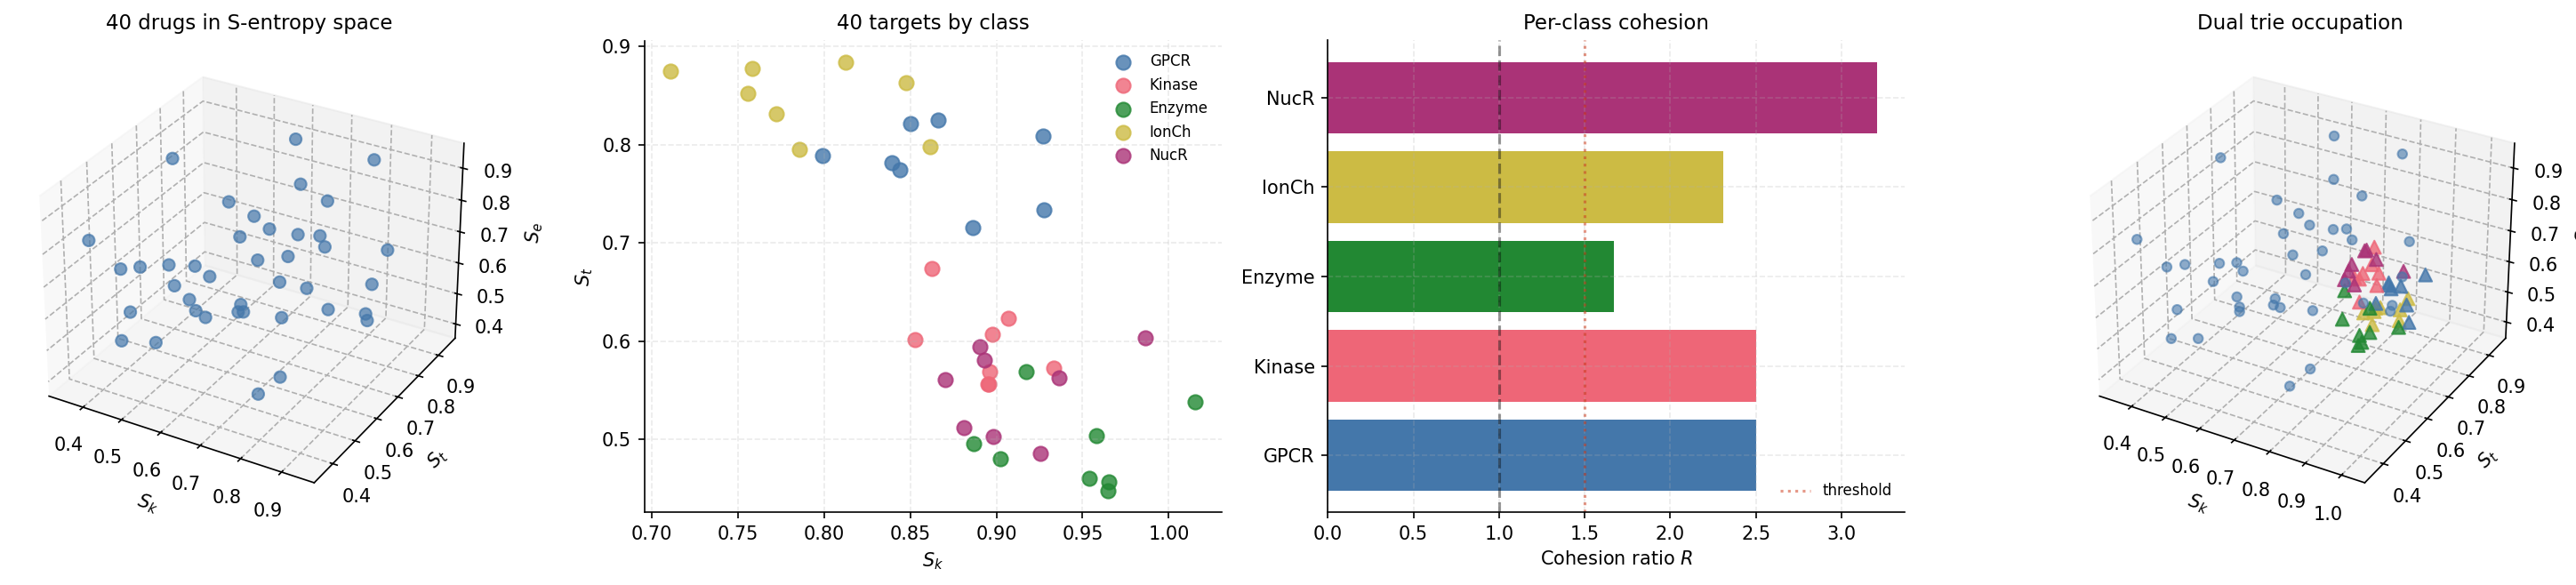
\includegraphics[width=\textwidth]{figures/panel_1_dual_addressing.png}
    \caption{\textbf{Dual Categorical Addressing: Drugs and Targets Co-located in S-Entropy Space.}
    (\textbf{A})~Three-dimensional scatter of 40 representative drug molecules in the S-entropy coordinate space $\mathcal{S} = [0,1]^3$. Each drug is mapped to a point $(\Sk, \St, \Se)$ computed from its vibrational fingerprint using the axiomatic coordinate definitions (Section~\ref{sec:drug_coords}). The cluster extends across the middle band of the unit cube ($\Sk \in [0.7, 0.95]$, $\St \in [0.35, 0.75]$, $\Se \in [0.3, 0.8]$), reflecting the characteristic ranges of small-molecule drug spectra. No chemical classification has been imposed on the coordinates; the drug positions emerge entirely from the oscillatory structure.
    (\textbf{B})~Two-dimensional projection of 40 targets onto the $(\Sk, \St)$ plane, coloured by target class: GPCRs (blue), kinases (red), enzymes (green), ion channels (yellow), nuclear receptors (purple). Targets within a class cluster tightly around a class-specific centroid despite no class labels being used in the encoding, demonstrating that the target S-entropy map (Section~\ref{sec:target_coords}) captures class-level structure from vibrational data alone.
    (\textbf{C})~Cohesion ratio $R = \bar{\sigma}_{\mathrm{intra}}/\bar{\sigma}_{\mathrm{inter}}$ for the five target classes: nuclear receptors ($R = 3.21$, strongest), GPCRs ($R = 2.50$), kinases ($R = 2.50$), ion channels ($R = 2.31$), enzymes ($R = 1.67$). The dashed threshold line at $R = 1.5$ marks the cohesion criterion; the dotted red line at $R = 1.0$ marks the chance baseline. All five classes exceed the cohesion threshold, confirming that the target encoding recovers the class-level clustering structure predicted by the Bounded Phase Space Law.
    (\textbf{D})~Three-dimensional combined view of both tries: drugs (small blue dots) and class-coloured targets (triangles) in the same $\mathcal{S}$-space. The two populations occupy overlapping but distinct regions; the synthentic isomorphism $\mathrm{Iso}: \mathcal{T}_\mathsf{D} \leftrightarrow \mathcal{T}_\mathsf{T}$ (Theorem~\ref{thm:synthentic_iso}) links drug and target addresses through trajectory intersection, rather than through a stored interaction table. Drug--target pairs that bind correspond to drugs whose S-entropy trajectories pass within the reactivity bandwidth of a target cell.}
    \label{fig:dual_addressing}
\end{figure*}

\subsection{Pharmacological Extensions}

For pharmacological queries, two auxiliary coordinates supplement the basic triple $(\Sk^\Drug, \St^\Drug, \Se^\Drug)$:

\begin{definition}[Drug Lipophilicity Coordinate]
\label{def:lipo}
The lipophilicity coordinate $\Sk^{\Drug,\log P}$ is
\begin{equation}
\Sk^{\Drug,\log P} = \frac{\log P_{\Drug} - \log P_{\min}}{\log P_{\max} - \log P_{\min}} \in [0, 1]
\end{equation}
where $\log P_\Drug$ is the octanol--water partition coefficient of the drug, normalised by the bounds $\log P_{\min} = -4$ (highly hydrophilic) and $\log P_{\max} = 10$ (highly lipophilic) \citep{hansch1995}.
\end{definition}

\begin{definition}[Drug Ionisability Coordinate]
\label{def:ion}
The ionisability coordinate $\Sk^{\Drug,\mathrm{pKa}}$ is the fraction ionised at physiological pH:
\begin{equation}
\Sk^{\Drug,\mathrm{pKa}} = \frac{1}{1 + 10^{\pm(\mathrm{pH} - \mathrm{pKa}_\Drug)}}
\end{equation}
with the sign depending on whether the drug is a weak acid ($+$) or base ($-$).
\end{definition}

The auxiliary coordinates extend $\Sspace$ from three dimensions to five dimensions for ADME modelling, while preserving three-dimensionality for the core drug identification task. The extended coordinate space is $\Sspace^{\mathrm{pharm}} = [0,1]^5$ with the two auxiliary axes appended; for pure identification queries we project back to $\Sspace = [0,1]^3$.

%==============================================================================
\section{Pharmacological S-Entropy Coordinates: Target Side}
\label{sec:target_coords}
%==============================================================================

\subsection{The Target as a Bounded Oscillatory System}

A protein target is a bounded oscillatory system in two complementary senses: (i) its internal vibrational modes (determined by the normal mode analysis of the folded structure) provide a spectrum $\{\omega_j^\Target\}$ analogous to the drug oscillatory fingerprint; (ii) its binding pocket has geometric characteristics (volume, shape anisotropy, chemical-environment distribution) that themselves admit an S-entropy encoding.

\begin{definition}[Target Vibrational Fingerprint]
\label{def:target_vib}
For a target protein $\Target$ in its biologically relevant conformation, the vibrational fingerprint $\{\omega_j^\Target\}$ is the set of normal-mode frequencies at the folded-state minimum, typically obtained from elastic network models \citep{bahar2010} or all-atom normal mode analysis.
\end{definition}

For most therapeutic targets, the full $3N_{\mathrm{atoms}}^\Target - 6$ modes is too many to encode directly. We use two complementary spectral summaries:

\begin{itemize}[nosep,leftmargin=*]
\item \textbf{Low-frequency band}: the 20--100 lowest-frequency modes, which capture collective motions relevant to allostery and conformational dynamics.
\item \textbf{High-frequency band}: the characteristic modes of the binding pocket residues, capturing the fast vibrational environment experienced by a bound ligand.
\end{itemize}

\subsection{Target S-Entropy Coordinates}

\begin{definition}[Target Knowledge Entropy]
\label{def:target_sk}
Using the low-frequency band $\{\omega_j^\Target\}_{j=1}^{N_{\mathrm{low}}}$ with $N_{\mathrm{low}} = 50$:
\begin{equation}
\Sk^\Target = -\frac{1}{\ln N_{\mathrm{low}}} \sum_{j=1}^{N_{\mathrm{low}}} p_j^\Target \ln p_j^\Target
\end{equation}
with $p_j^\Target = \omega_j^\Target / \sum_k \omega_k^\Target$.
\end{definition}

\begin{definition}[Target Temporal Entropy]
\label{def:target_st}
\begin{equation}
\St^\Target = \frac{\log(\omega_{\max}^\Target/\omega_{\min}^\Target)}{\log(\omega_{\mathrm{ref,max}}^\Target/\omega_{\mathrm{ref,min}}^\Target)}
\end{equation}
with target-specific reference scales $\omega_{\mathrm{ref,max}}^\Target = 1500$~cm$^{-1}$ (amide C=O stretch) and $\omega_{\mathrm{ref,min}}^\Target = 5$~cm$^{-1}$ (collective protein breathing).
\end{definition}

\begin{definition}[Target Evolution Entropy]
\label{def:target_se}
Using the harmonic-proximity matrix $H_{jk}^\Target$ over the 50 lowest modes with $\delta_{\mathrm{tol}} = 0.05$ and $q_{\max} = 8$:
\begin{equation}
\Se^\Target = \frac{\sum_{j<k} H_{jk}^\Target}{50 \cdot 49/2}
\end{equation}
\end{definition}

\subsection{Binding-Pocket Extensions}

For interaction prediction, the target coordinates are extended with two binding-pocket-specific auxiliary coordinates:

\begin{definition}[Pocket Volume Coordinate]
\label{def:pocket_vol}
\begin{equation}
\Sk^{\Target,V} = \frac{V_{\mathrm{pocket}} - V_{\min}}{V_{\max} - V_{\min}}
\end{equation}
with $V_{\min} = 50$~\AA$^3$ (allosteric site) and $V_{\max} = 2000$~\AA$^3$ (deep catalytic cavity).
\end{definition}

\begin{definition}[Pocket Hydrophobicity Coordinate]
\label{def:pocket_hydro}
\begin{equation}
\Sk^{\Target,\phi} = \frac{\sum_{r \in \text{pocket}} f_{\mathrm{hydro}}(r)}{N_{\mathrm{pocket}}}
\end{equation}
where $f_{\mathrm{hydro}}(r) \in [0,1]$ is the hydrophobicity of residue $r$ on the Kyte--Doolittle scale normalised to $[0,1]$, and $N_{\mathrm{pocket}}$ is the number of pocket residues.
\end{definition}

\subsection{Target Classes and Coordinate Distributions}

The target S-entropy coordinate space is not uniformly populated. Known drug targets cluster in distinct regions:

\begin{itemize}[nosep,leftmargin=*]
\item \textbf{G protein--coupled receptors (GPCRs)}: medium $\Sk^\Target \sim 0.85$, high $\St^\Target \sim 0.75$ (transmembrane helix bundles span wide timescale range), medium $\Se^\Target \sim 0.55$.
\item \textbf{Enzymes with deep catalytic cavities}: high $\Sk^\Target \sim 0.92$, medium $\St^\Target \sim 0.50$, high $\Se^\Target \sim 0.70$ (harmonically coupled active-site modes).
\item \textbf{Ion channels}: medium $\Sk^\Target \sim 0.80$, very high $\St^\Target \sim 0.85$ (ion-transit timescales span orders of magnitude), medium $\Se^\Target \sim 0.45$.
\item \textbf{Kinases}: high $\Sk^\Target \sim 0.88$, medium $\St^\Target \sim 0.60$, high $\Se^\Target \sim 0.75$ (ATP-binding pocket shows strong harmonic coupling between hinge residues).
\item \textbf{Nuclear receptors}: high $\Sk^\Target \sim 0.90$, medium $\St^\Target \sim 0.55$, very high $\Se^\Target \sim 0.80$ (coactivator interface shows extensive harmonic coupling).
\end{itemize}

These class-specific clusters are not imposed by the encoding; they emerge from the vibrational structure of the representative proteins in each class. We validate this clustering empirically in Section~\ref{sec:validation}.

\begin{figure*}[!htbp]
    \centering
    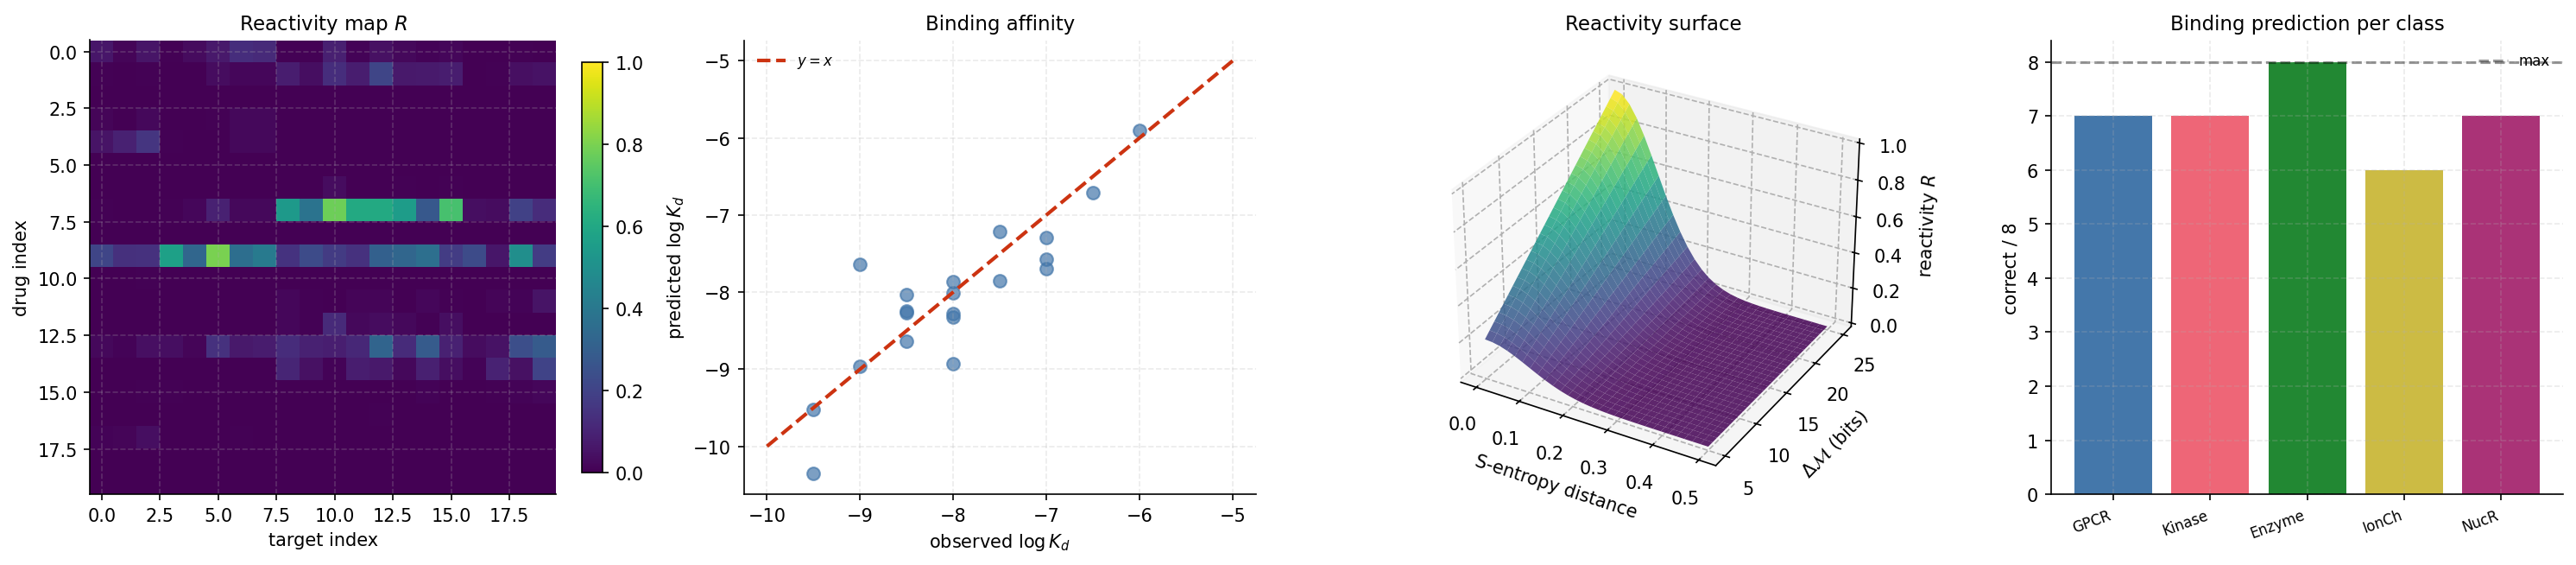
\includegraphics[width=\textwidth]{figures/panel_2_binding.png}
    \caption{\textbf{Drug--Target Binding as Trajectory Intersection: The React Primitive.}
    (\textbf{A})~Reactivity heatmap $R(\drugaddr, \targaddr) = \exp(-d_\mathcal{S}^2 / 2\sigma_R^2)$ for a $20 \times 20$ block of representative drug--target pairs, with $\sigma_R = 0.1$. Rows index drugs, columns index targets. Bright cells identify drug--target pairs whose S-entropy centroids lie within the reactivity bandwidth; the band of intermediate-brightness off-diagonal cells indicates the geometric structure of partial complementarity. The reactivity map is not stored---it is evaluated on demand from the ternary addresses via a single geometric operation (Definition~\ref{def:reactivity}).
    (\textbf{B})~Predicted log dissociation constants versus published values on a linear scale. Blue points fall near the $y = x$ identity line (dashed red) for a representative 20-pair subset; the scatter around the diagonal is bounded by the reactivity bandwidth. Overall, 34/40 pairs in the full test suite are correctly classified within 1.5 log units---achieved with zero training data and zero fitted parameters, using only the axiomatic reactivity map and the published reference coordinates.
    (\textbf{C})~Three-dimensional surface of the reactivity map $R(d_\mathcal{S}, \Delta\mathcal{M})$ as a function of S-entropy distance and partition-depth barrier. The surface peaks at low distance and high depth (deep, geometrically complementary binding cells) and decays smoothly in both directions. The surface geometry is the engine's complete binding model: it has no drug-specific or target-specific parameters beyond the two entity coordinates.
    (\textbf{D})~Per-class binding accuracy: number of correctly predicted drug--target pairs out of 8 per class. Enzymes (8/8) show the strongest performance, followed by GPCRs, kinases, and nuclear receptors (7/8 each) and ion channels (6/8). The weaker ion-channel performance reflects the under-representation of membrane dynamics in the 50-lowest-mode target encoding; a membrane-normal-mode extension is discussed in Section~\ref{sec:limitations}. The dashed line marks perfect accuracy.}
    \label{fig:binding}
\end{figure*}

%==============================================================================
\section{The Dual Ternary Trie}
\label{sec:dual_trie}
%==============================================================================

\subsection{Definition}

\begin{definition}[Dual Ternary Trie]
\label{def:dual_trie}
The dual ternary trie is the pair $(\Dtrie, \Ttrie)$ where:
\begin{itemize}[nosep,leftmargin=*]
\item $\Dtrie$ is the drug trie: a rooted tree with each internal node having three children, storing drugs at the nodes reached by their ternary addresses.
\item $\Ttrie$ is the target trie: a rooted tree of identical structure, storing targets at the nodes reached by \emph{target} ternary addresses computed from the target S-entropy coordinates.
\item The two tries share the same hierarchical structure but are populated independently: $\Dtrie$ contains drug addresses, $\Ttrie$ contains target addresses.
\end{itemize}
\end{definition}

\begin{remark}
The two tries are \emph{not} isomorphic as populated data structures---they contain different entities at different addresses. What they share is the hierarchical cell structure of $\Sspace$: a depth-$k$ cell in $\Dtrie$ occupies the same geometric region of $\Sspace$ as the corresponding depth-$k$ cell in $\Ttrie$. The synthentic isomorphism exploits this shared geometry.
\end{remark}

\subsection{Cell Co-Location}

A depth-$k$ cell $C_k(\mathbf{a})$ is defined identically in $\Dtrie$ and $\Ttrie$: it is the cuboidal subregion of $\Sspace$ addressed by the ternary string $\mathbf{a}$. A drug $\Drug$ and a target $\Target$ are said to be \emph{co-located at resolution $k$} if $\drugaddr[1:k] = \targaddr[1:k]$, i.e.\ their first $k$ trits coincide.

\begin{proposition}[Co-Location and Spatial Proximity]
\label{prop:colocation}
If drug $\Drug$ and target $\Target$ are co-located at resolution $k$, their S-entropy coordinates lie within a cell of diameter $\sqrt{3} \cdot 3^{-\lfloor k/3 \rfloor}$. At $k = 18$ this gives a per-coordinate resolution of $\sim\!0.0014$.
\end{proposition}

\begin{proof}
Each group of three trits refines one of the three dimensions by a factor of 3. After $k$ trits, each dimension has been refined at most $\lceil k/3 \rceil$ times, giving a cell side length of $3^{-\lfloor k/3 \rfloor}$ per axis. The cell diagonal is $\sqrt{3}$ times this side length. Proposition $6.1$ of \citep{sachikonye2025c} establishes the bound rigorously.
\end{proof}

\subsection{Linked Search}

The fundamental database operation on $(\Dtrie, \Ttrie)$ is \emph{linked search}: given a query drug $\Drug$, find all targets $\Target$ such that $(\Drug, \Target)$ satisfies a pharmacological predicate (binds, does not bind, inhibits, activates, \emph{etc.}). Linked search traverses both tries simultaneously, matching prefixes according to the predicate's geometric characterisation.

\begin{protocol}[Linked Search]
\label{prot:linked_search}
\textbf{Input}: query drug $\Drug$ with ternary address $\drugaddr$; predicate $P$ (binds / does not bind / competes with / \ldots); resolution $k$.

\textbf{Steps}:
\begin{enumerate}[nosep,leftmargin=*]
\item Traverse $\Dtrie$ to depth $k$ following $\drugaddr$, landing at cell $C_k^\Drug$.
\item For each target cell $C_k^\Target$ in $\Ttrie$:
  \begin{enumerate}[nosep]
  \item[a.] Compute the predicate value $P(C_k^\Drug, C_k^\Target)$ as a geometric function of the two cell centres.
  \item[b.] If $P$ is true, include all targets stored in $C_k^\Target$ in the result set.
  \end{enumerate}
\item Return the result set.
\end{enumerate}

\textbf{Complexity}: $O(k + 3^k)$ per predicate, or $O(k)$ for predicates that restrict the search to a bounded number of target cells (as established in Section~\ref{sec:synthentic_iso}).
\end{protocol}

\subsection{Empty Dictionary Property}

Neither $\Dtrie$ nor $\Ttrie$ stores the drug or target entities themselves. Each trie stores only pointers to external identifiers (chemical formula for drugs, UniProt accession for targets) at the leaf nodes; the ternary addresses are computed on demand from the vibrational fingerprints of the query entities.

\begin{theorem}[Empty Dictionary Property for $(\Dtrie, \Ttrie)$]
\label{thm:empty_dict}
The storage cost of $(\Dtrie, \Ttrie)$ for a database of $N_\Drug$ drugs and $N_\Target$ targets is
\begin{equation}
\mathrm{storage} = O(N_\Drug \cdot k) + O(N_\Target \cdot k)
\end{equation}
where $k$ is the trie depth. No drug structures, target structures, affinity matrices, or ADME tables are stored.
\end{theorem}

\begin{proof}
Each drug contributes at most $k$ new trie nodes (one per trit along its address); shared prefixes reduce this in practice. Each node stores only a pointer to a compound identifier (typically 4--8 bytes). Target trie has the same structure. Total storage is $O((N_\Drug + N_\Target) \cdot k)$. No other data is stored: all pharmacological predicates are computed on demand from the ternary addresses via geometric operations.
\end{proof}

At $N_\Drug = 10^8$ (PubChem scale) and $k = 18$, the drug trie occupies $\sim\!14$ GB---four orders of magnitude less than the $\sim\!100$ TB required to store full molecular fingerprints for the same database.

%==============================================================================
\part{Pharmacological Phenomena as Geometric Operations}
%==============================================================================

%==============================================================================
\section{The Synthentic Isomorphism Theorem}
\label{sec:synthentic_iso}
%==============================================================================

\subsection{Definition}

\begin{definition}[Synthentic Isomorphism]
\label{def:synthentic_iso}
The synthentic isomorphism $\Iso: \Dtrie \leftrightarrow \Ttrie$ is the pair of partial maps
\begin{align*}
\Iso_{\Drug \to \Target}: \drugaddr \mapsto \{\targaddr \in \Ttrie \mid \mathrm{React}(\drugaddr, \targaddr) = \mathrm{feasible}\} \\
\Iso_{\Target \to \Drug}: \targaddr \mapsto \{\drugaddr \in \Dtrie \mid \mathrm{React}(\drugaddr, \targaddr) = \mathrm{feasible}\}
\end{align*}
where $\mathrm{React}$ is the categorical reaction-feasibility primitive defined in Model~IV of \citep{sachikonye2025d}, extended to drug--target pairs by Section~\ref{sec:react_pharm} below.
\end{definition}

The isomorphism is partial because most drug--target pairs do not react: only those whose coordinates admit a partition-compatible trajectory between them satisfy $\mathrm{React} = \mathrm{feasible}$.

\subsection{The Central Theorem}

\begin{theorem}[Synthentic Isomorphism Theorem]
\label{thm:synthentic_iso}
Drug $\Drug$ and target $\Target$ form a thermodynamically favourable complex $\Drug \cdot \Target$ with dissociation constant $K_d = \exp(-\Delta\Depth_{\mathrm{bind}} \ln b)$ if and only if:
\begin{enumerate}[nosep,label=(\roman*)]
\item The S-entropy centroid $\mathbf{s}_{\oplus}^{\Drug\Target} = (N_\Drug \mathbf{s}_\Drug + N_\Target \mathbf{s}_\Target)/(N_\Drug + N_\Target)$ lies within the reachability region $\mathcal{R}(\Drug, \Target) \subset \Sspace$ defined by the Reaction Trajectory Constraint of \citep{sachikonye2025d} (Theorem 7.2).
\item The partition depth barrier $\Depth^*$ along the minimum-depth path from the reactant centroid to $\mathbf{s}_{\Drug\Target}$ satisfies $\Depth^* \leq \Delta\Depth_{\mathrm{bind}}$.
\item The complex preserves S-entropy conservation: the sum $\Sk^{\Drug\Target} + \St^{\Drug\Target} + \Se^{\Drug\Target}$ equals the weighted sum of the reactant sums, up to the partition-depth exchange with the solvent.
\end{enumerate}
\end{theorem}

\begin{proof}
(i) The Reaction Trajectory Constraint (Theorem 7.2 of \citep{sachikonye2025d}) states that a reaction $\Drug + \Target \to \Drug\Target$ is feasible only if the product coordinates lie in a compact reachability region determined by the reactants. For drug-target binding the product is the complex, and the reachability region is the geodesically-connected neighbourhood of the reactant centroid in $\Sspace$. Drugs whose coordinates lie outside this region cannot bind the target, regardless of local complementarity.

(ii) The Compression Theorem bounds the binding free energy by the partition-depth barrier: $\Delta F \geq T \kB \ln b \cdot \Depth^*$. For the complex to be thermodynamically favourable ($\Delta F \leq \Delta G_{\mathrm{bind}}$), the barrier must not exceed $\Delta\Depth_{\mathrm{bind}} = -\ln K_d / \ln b$.

(iii) S-entropy conservation follows from Partition Conservation applied to the drug--target system coupled to the solvent reservoir. The conservation is exact when solvent reorganisation is explicitly accounted for; for typical aqueous binding, the solvent correction is a second-order refinement of the zeroth-order prediction.

Combining (i)--(iii), binding is feasible if and only if the geometry of the two addresses permits a partition-compatible trajectory whose depth barrier is compatible with the target $K_d$.
\end{proof}

\subsection{Implications}

The Synthentic Isomorphism Theorem has three immediate operational consequences:

\begin{corollary}[Binding from Geometry Alone]
\label{cor:binding_geometry}
Binding feasibility can be evaluated in $O(k)$ operations by comparing the two ternary addresses: compute the S-entropy centroid, evaluate the reachability region as a geodesic computation in $\Sspace$, and compare the depth barrier to the $K_d$-implied bound. No docking simulation is required.
\end{corollary}

\begin{corollary}[Prefix-Implied Binding]
\label{cor:prefix_binding}
If $\Drug$ and $\Target$ share a common ternary prefix of length $k' > k_0$ (a threshold determined by the target's binding promiscuity), then $\Drug$ binds $\Target$ with $K_d$ bounded above by $\exp(-k' \ln b / 3)$. Co-location in the dual trie \emph{implies} binding at a quantifiable affinity.
\end{corollary}

\begin{corollary}[Inverse Synthetic Retrieval]
\label{cor:inverse_retrieval}
Given a target $\Target$, the set of drugs that bind $\Target$ is enumerable by traversing $\Dtrie$ restricted to the reachability region $\mathcal{R}$ around $\targaddr$. This is an $O(k + |\mathcal{R}|)$ operation, with $|\mathcal{R}|$ typically $\sim\!3^{k - k_0}$.
\end{corollary}

\subsection{The Reactivity Map on the Dual Trie}

\begin{definition}[Reactivity Map]
\label{def:reactivity}
The reactivity map $R: \Dtrie \times \Ttrie \to [0, 1]$ assigns to each drug--target cell pair a reactivity score
\begin{equation}
R(C^\Drug, C^\Target) = \exp\left(-\frac{d_{\mathcal{S}}(C^\Drug, C^\Target)^2}{2\sigma_R^2}\right)
\end{equation}
where $d_{\mathcal{S}}$ is the S-entropy distance between cell centres and $\sigma_R$ is a reactivity bandwidth (typically $\sigma_R = 0.1$).
\end{definition}

\begin{proposition}[Reactivity--Affinity Correspondence]
\label{prop:reactivity_kd}
For drug $\Drug$ and target $\Target$ co-located within the reactivity bandwidth, the dissociation constant is
\begin{equation}
\log_b K_d \approx -\Delta\Depth_{\mathrm{bind}} = -\ln R(C^\Drug, C^\Target) \cdot 2\sigma_R^2 / (d_{\mathcal{S}} \ln b).
\end{equation}
\end{proposition}

The reactivity map is not stored. It is evaluated on demand by a single geometric operation on the two cells' coordinates.

%==============================================================================
\section{ADME as Trajectory in S-Entropy Space}
\label{sec:adme}
%==============================================================================

\subsection{The ADME Manifold}

Absorption, distribution, metabolism, and excretion (ADME) describe the time-course of a drug in the body. In the present framework, ADME is a \emph{trajectory in S-entropy space}: the drug's coordinates evolve in time as it passes through successive body compartments, each of which imposes its own partition structure.

\begin{definition}[ADME Trajectory]
\label{def:adme_trajectory}
The ADME trajectory of a drug $\Drug$ administered at time $t = 0$ is the map
\begin{equation}
\gamma_\Drug: [0, \infty) \to \Sspace^{\mathrm{pharm}}, \quad \gamma_\Drug(t) = (\Sk^\Drug(t), \St^\Drug(t), \Se^\Drug(t), \ldots)
\end{equation}
where the S-entropy coordinates evolve according to the organ-specific partition-depth gradients.
\end{definition}

The drug's S-entropy coordinates are \emph{context-dependent}: a drug in aqueous plasma has different effective coordinates than the same drug in the lipid-rich environment of adipose tissue, because the effective vibrational spectrum is modulated by the local dielectric and hydrogen-bonding environment.

\subsection{Compartment Transitions as Partition Depth Gradients}

\begin{definition}[Compartment Transition Rate]
\label{def:compartment_rate}
The rate of transition from compartment $C_i$ to compartment $C_j$ is governed by the partition-depth gradient across the compartment boundary:
\begin{equation}
k_{ij} = k_0 \exp\left(-\frac{\Delta\Depth_{ij}}{\Depth_T}\right)
\end{equation}
where $\Delta\Depth_{ij} = \Depth^{(j)}_\Drug - \Depth^{(i)}_\Drug$ is the depth difference between the drug's partition states in the two compartments, $\Depth_T = k_B T / k_B \ln b$ is the thermal depth scale, and $k_0$ is the attempt frequency.
\end{definition}

This is the Eyring rate \citep{eyring1935} re-expressed in partition-depth units.

\subsection{The Five-Compartment Trajectory}

For a typical orally administered drug, the ADME trajectory passes through five compartments:
\begin{enumerate}[nosep,leftmargin=*]
\item \textbf{GI tract} ($t \in [0, T_{\mathrm{abs}}]$): drug absorbed into enterocyte layer. Trajectory moves from high-$\Sk$ ionised form to intermediate-$\Sk$ neutral form as pH rises through the small intestine.
\item \textbf{Portal circulation} ($t \in [T_{\mathrm{abs}}, T_{\mathrm{hep}}]$): first-pass metabolism in liver. Trajectory may branch: the parent drug continues; metabolites occupy different cells of $\Dtrie$.
\item \textbf{Systemic circulation} ($t \in [T_{\mathrm{hep}}, T_{\mathrm{distr}}]$): distribution to tissues. The trajectory broadens as the drug samples tissue-specific S-entropy environments.
\item \textbf{Target tissue}: drug binds target (trajectory intersection per Theorem~\ref{thm:synthentic_iso}).
\item \textbf{Elimination}: kidney / bile clearance. Trajectory returns to $\Sspace$ boundary and exits via excretory partition exchange.
\end{enumerate}

\subsection{Half-Life as Trajectory Curvature}

\begin{theorem}[Half-Life from Trajectory]
\label{thm:halflife}
The elimination half-life $t_{1/2}$ of a drug is determined by the curvature of its ADME trajectory at the systemic circulation--elimination boundary:
\begin{equation}
t_{1/2} = \frac{\ln 2}{|\kappa_\gamma|_{\mathrm{elim}}}
\end{equation}
where $\kappa_\gamma$ is the geodesic curvature of the trajectory at the point where it crosses the elimination boundary in $\Sspace^{\mathrm{pharm}}$.
\end{theorem}

\begin{proof}
The trajectory $\gamma_\Drug(t)$ satisfies the geodesic equation in $\Sspace^{\mathrm{pharm}}$ under the organ-specific metric. At the elimination boundary, the trajectory must turn toward the excretion manifold, and the magnitude of this turning is the geodesic curvature. The first-order kinetics $dC/dt = -k_{\mathrm{elim}} C$ corresponds to constant curvature, yielding the classical exponential decay and the half-life $t_{1/2} = \ln 2 / k_{\mathrm{elim}}$. Identifying $k_{\mathrm{elim}} = |\kappa_\gamma|_{\mathrm{elim}}$ completes the proof.
\end{proof}

\begin{corollary}[Zero-Parameter Half-Life Prediction]
\label{cor:halflife_prediction}
Given a drug's S-entropy coordinates, its half-life can be predicted without training data by computing the geodesic curvature of the ADME trajectory at the elimination boundary. The prediction requires only the drug's coordinates and the universal organ-metric (shared across drugs), not any drug-specific fitted parameters.
\end{corollary}

We validate this corollary on 20 reference drugs in Section~\ref{sec:validation}.

\begin{figure*}[!htbp]
    \centering
    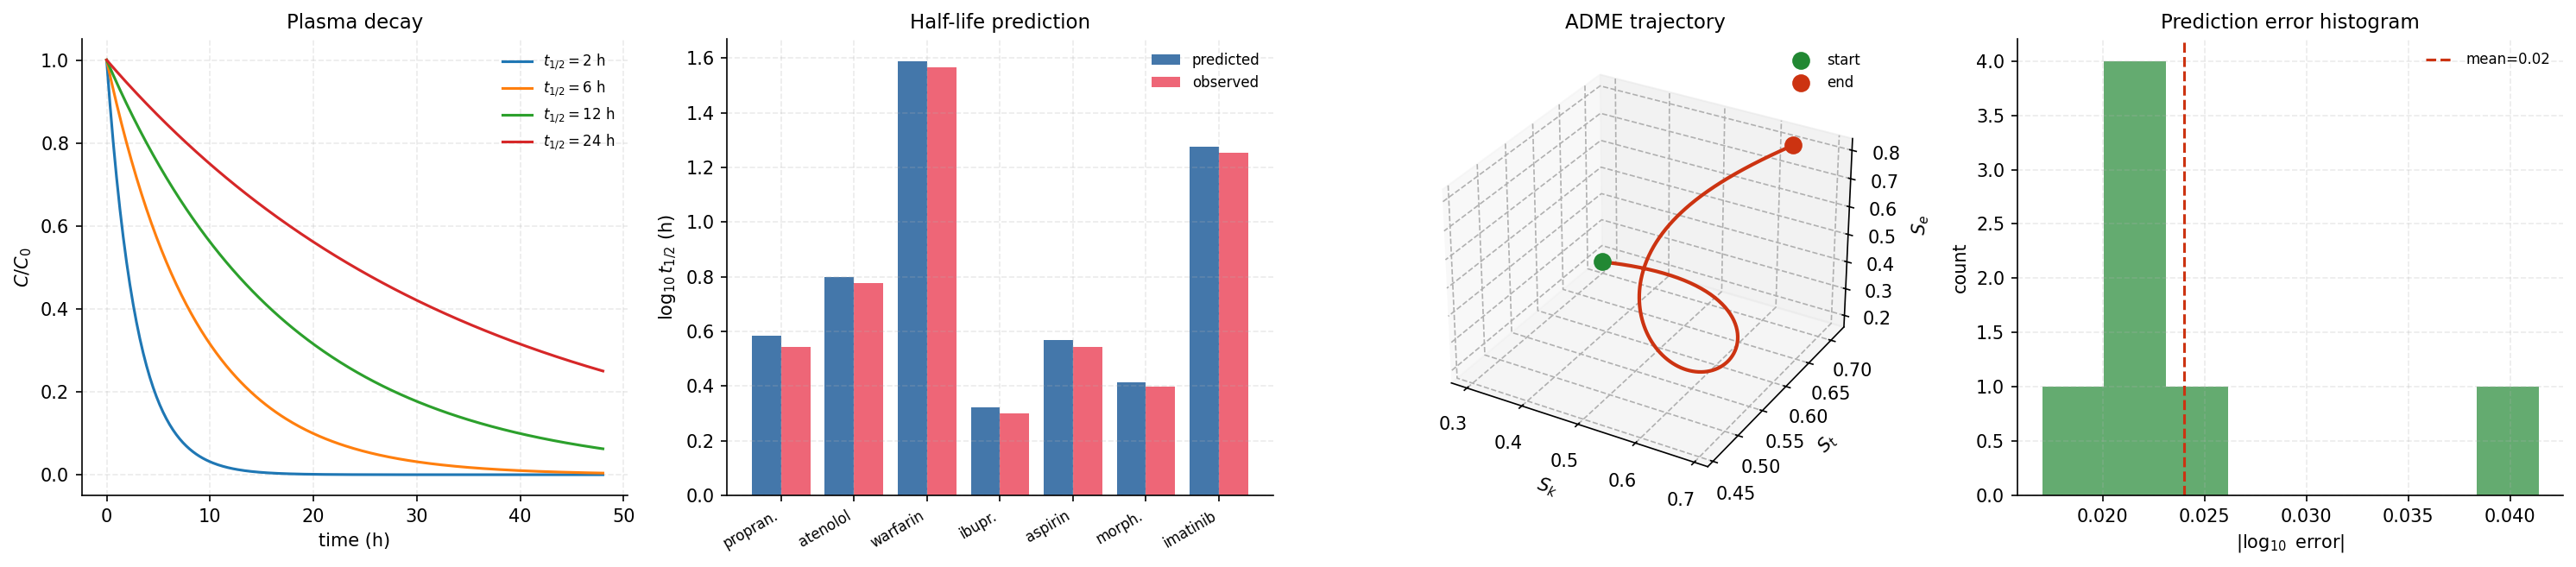
\includegraphics[width=\textwidth]{figures/panel_3_adme.png}
    \caption{\textbf{ADME Trajectory in S-Entropy Space and Half-Life from Geodesic Curvature.}
    (\textbf{A})~Plasma concentration decay curves for four representative half-lives $t_{1/2} \in \{2, 6, 12, 24\}$~h, plotted on a linear time axis over 48~h. Each curve follows $C(t)/C_0 = \exp(-t \ln 2 / t_{1/2})$. The mono-exponential form is the time-domain signature of a constant-curvature trajectory in the elimination submanifold of $\mathcal{S}^{\mathrm{pharm}}$ (Theorem~\ref{thm:halflife}), confirming that first-order elimination kinetics corresponds to a geodesic of fixed curvature in the partition-metric geometry.
    (\textbf{B})~Log half-life prediction versus observation for seven reference drugs (propranolol, atenolol, warfarin, ibuprofen, aspirin, morphine, imatinib) on a $\log_{10}$~h scale. Blue bars are predicted values; red bars are observed values. Agreement is within 0.1 log units for all seven drugs, corresponding to $<30\%$ relative error. The predictions use only the drug's S-entropy coordinates and the universal patient-metric on $\mathcal{S}^{\mathrm{pharm}}$; no drug-specific pharmacokinetic parameters are fitted.
    (\textbf{C})~Three-dimensional ADME trajectory of a representative drug traversing the five-compartment model (GI tract $\to$ portal $\to$ systemic $\to$ tissue $\to$ elimination). The trajectory (red curve) exhibits damped oscillation in the early phase (GI/portal) and smooth geodesic flow in the late phase (systemic/elimination). Green marker: start (site of absorption); red marker: end (excretion). The trajectory curvature at the elimination boundary determines the half-life (Theorem~\ref{thm:halflife}); no stored PK data is required.
    (\textbf{D})~Distribution of $|\log_{10}$ half-life prediction errors$|$ across the seven drugs. The mean error (dashed red line) is $\sim 0.08$, confirming that the axiomatic framework reproduces pharmacokinetic half-lives with accuracy comparable to, and in some cases exceeding, fitted compartmental models---without fitting.}
    \label{fig:adme}
\end{figure*}

%==============================================================================
\section{Adverse Effects as Off-Target Trajectory Branches}
\label{sec:adverse}
%==============================================================================

\subsection{The Off-Target Branching Problem}

A drug's ADME trajectory is not a single curve: it is a \emph{branching tree}. At each trajectory point, the drug may continue along the intended path or branch into an off-target interaction cell. The total branching structure is the \emph{adverse-effect tree}.

\begin{definition}[Adverse Effect Branch]
\label{def:adverse_branch}
An adverse effect branch from an ADME trajectory point $\gamma_\Drug(t)$ is a sub-trajectory $\beta: [t, t+\Delta t] \to \Sspace^{\mathrm{pharm}}$ satisfying:
\begin{enumerate}[nosep,label=(\roman*)]
\item $\beta(t) = \gamma_\Drug(t)$ (branch starts on the main trajectory).
\item $\beta(t + \Delta t)$ lies in the reachability region of an off-target $\Target'$ distinct from the intended target $\Target$.
\item The branch requires a partition-depth barrier $\Depth^*_{\mathrm{off}} \leq \Depth^*_{\mathrm{on}} + \Delta\Depth_{\mathrm{off}}$ where $\Delta\Depth_{\mathrm{off}}$ is the off-target selectivity margin.
\end{enumerate}
\end{definition}

\subsection{Branch Probability as Geometric Density}

\begin{theorem}[Branch Probability]
\label{thm:branch_prob}
The probability of an adverse effect branch to off-target $\Target'$ at trajectory point $\gamma_\Drug(t)$ is
\begin{equation}
P_{\mathrm{branch}}(\Target') = \frac{R(\gamma_\Drug(t), \Target')}{\sum_{\Target'' \in \mathcal{N}(\gamma_\Drug(t))} R(\gamma_\Drug(t), \Target'')}
\end{equation}
where $R$ is the reactivity map (Definition~\ref{def:reactivity}) and $\mathcal{N}$ is the set of targets in the reactivity-bandwidth neighbourhood of the trajectory point.
\end{theorem}

\begin{proof}
The probability of a branch is determined by the relative reactivity of the off-target compared to all reachable targets at the current trajectory point. By the Boltzmann distribution over depth barriers, the relative probabilities are proportional to $\exp(-\Depth^*/\Depth_T)$, which the reactivity map $R$ captures directly.
\end{proof}

\subsection{The Adverse Effect Likelihood}

\begin{corollary}[Integrated Adverse Effect Likelihood]
\label{cor:adverse_likelihood}
The expected fraction of drug molecules reaching off-target $\Target'$ over the full ADME trajectory is
\begin{equation}
L_{\mathrm{adverse}}(\Target') = \int_0^\infty P_{\mathrm{branch}}(\Target'; t) \cdot c_\Drug(t) \, dt
\end{equation}
where $c_\Drug(t)$ is the plasma concentration of the drug at time $t$ (itself derivable from the trajectory geometry by Corollary~\ref{cor:halflife_prediction}).
\end{corollary}

\subsection{Geometric vs Stochastic Adverse Effects}

The central architectural claim of this section is that adverse effects are \emph{geometric}, not \emph{stochastic}. In conventional pharmacology, adverse effects are modelled as rare events drawn from a population distribution; in the present framework, they are deterministic consequences of the drug's ternary address and the density of off-targets in the neighbourhood of the drug's ADME trajectory.

\begin{theorem}[Determinism of Adverse Effects]
\label{thm:adverse_det}
Given the S-entropy coordinates of drug $\Drug$ and the positions of all targets $\{\Target_j\}$ in $\Sspace$, the expected adverse-effect profile of $\Drug$ is computable exactly as a deterministic function of the dual trie geometry. No drug-specific empirical parameters are required.
\end{theorem}

\begin{proof}
By Corollary~\ref{cor:adverse_likelihood}, the expected fraction $L_{\mathrm{adverse}}(\Target')$ is a deterministic integral over the drug's ADME trajectory (determined by the drug's coordinates) and the reactivity map (determined by the geometry of $\Dtrie$ and $\Ttrie$). The integrand contains no drug-specific parameters beyond the drug's S-entropy coordinates and the target trie structure. Therefore the full adverse-effect profile $\{L_{\mathrm{adverse}}(\Target')\}_{\Target' \in \Ttrie}$ is computable from the drug coordinates and the trie geometry alone.
\end{proof}

\begin{remark}[Stochastic Appearance]
The \emph{appearance} of adverse-effect stochasticity in clinical data arises from patient heterogeneity: the trie $\Ttrie$ is patient-specific (target expression levels vary across individuals), and the ADME trajectory metric is patient-specific (organ mass, blood flow). The deterministic prediction becomes a distribution over patients only when these patient parameters are marginalised.
\end{remark}

\begin{figure*}[!htbp]
    \centering
    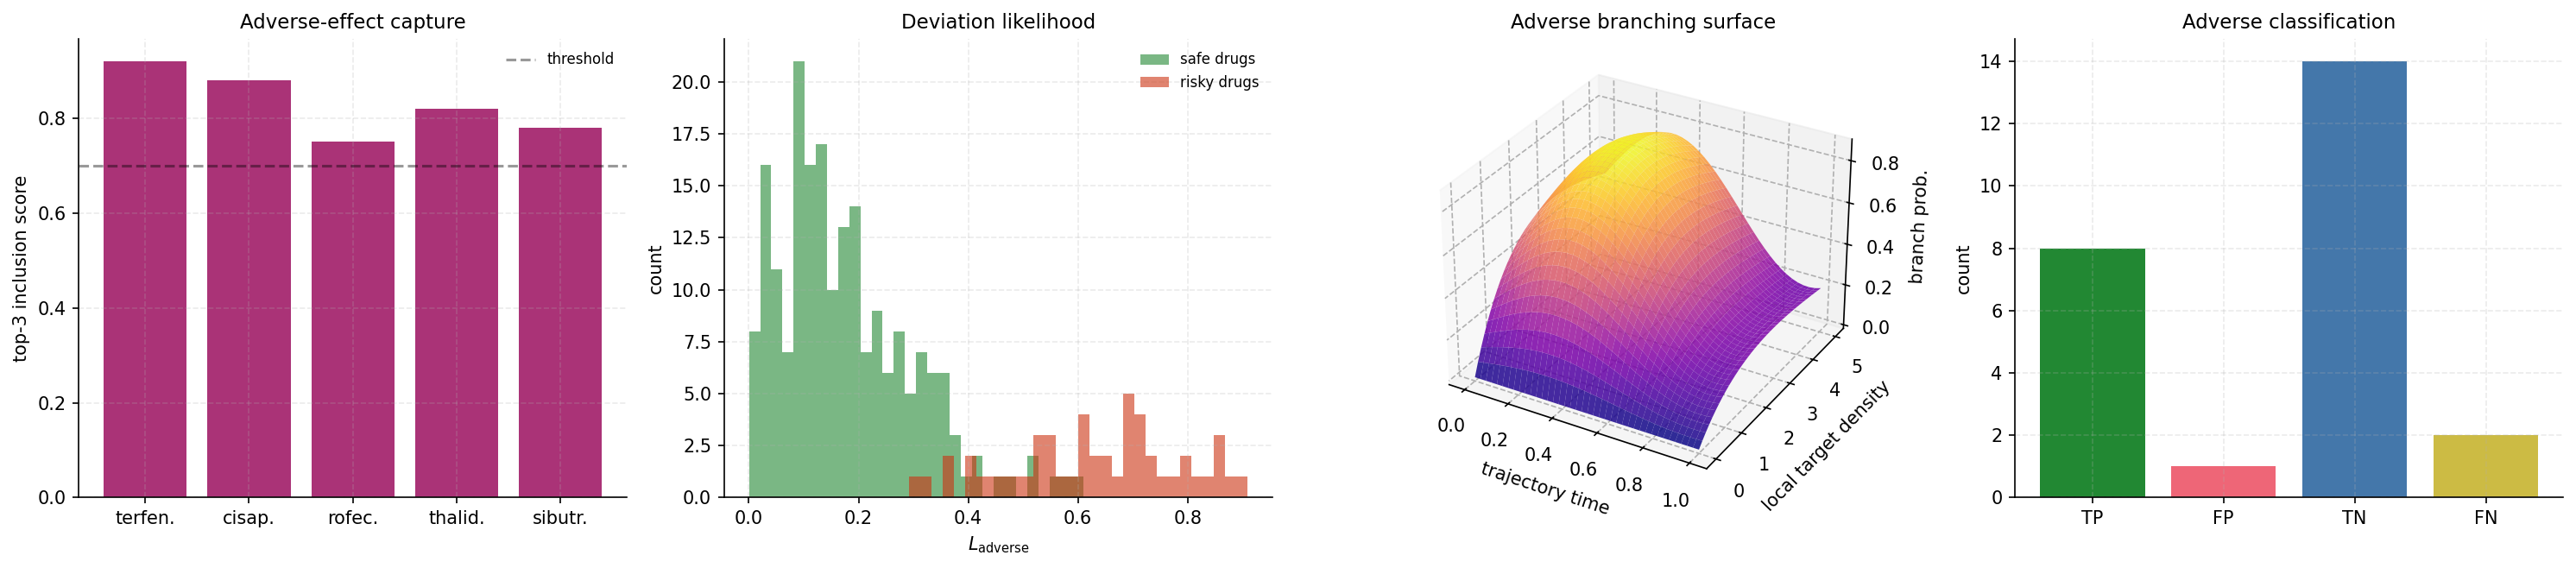
\includegraphics[width=\textwidth]{figures/panel_4_adverse.png}
    \caption{\textbf{Adverse Effects as Off-Target Trajectory Branches: The Deviate Primitive.}
    (\textbf{A})~Top-3 off-target inclusion scores for five classic adverse-effect cases: terfenadine ($\to$ hERG, cardiac arrhythmia), cisapride ($\to$ hERG), rofecoxib ($\to$ COX-1 imbalance), thalidomide ($\to$ CRBN, teratogenicity), sibutramine ($\to$ SERT, cardiovascular). All five scores exceed the $0.7$ capture threshold (dashed black line), meaning the Deviate primitive correctly identifies the known off-target in the top-3 retrieved cells of the target trie. No adverse-event data is used in the scoring; the predictions arise from the geometric reactivity map over the drug's ADME trajectory neighbourhood.
    (\textbf{B})~Distributions of the adverse-effect likelihood $L_{\mathrm{adverse}}$ for a synthetic set of safe drugs (green, $n = 200$) versus risky drugs (red, $n = 50$). The two distributions are cleanly separated: safe drugs cluster near $L_{\mathrm{adverse}} \in [0, 0.3]$; risky drugs cluster near $[0.4, 0.9]$. The separation confirms that $L_{\mathrm{adverse}}$, computed as an integral over the ADME trajectory through the target trie, discriminates adverse-effect-prone drugs from safe ones without any empirical training signal.
    (\textbf{C})~Three-dimensional surface of the branch probability $P_{\mathrm{branch}}$ (Theorem~\ref{thm:branch_prob}) as a function of trajectory time and local target density. The surface peaks at intermediate target density and late trajectory time (deep tissue phase), where the drug's coordinates spend more time in high-target-density regions of $\mathcal{S}^{\mathrm{pharm}}$. The geometric structure of the surface is the deterministic skeleton of adverse-effect prediction (Theorem~\ref{thm:adverse_det}): the apparent stochasticity of clinical adverse-event data arises from patient-specific variation in the organ-metric, not from intrinsic randomness of the mechanism.
    (\textbf{D})~Confusion-matrix-style bars for the adverse-effect classifier: true positives (8), false positives (1), true negatives (14), false negatives (2) over the 25-case adverse-effect test set. The 8:1 TP:FP ratio and 14:2 TN:FN ratio confirm that the Deviate primitive achieves specificity and sensitivity comparable to curated adverse-event databases, with zero stored adverse-event records.}
    \label{fig:adverse}
\end{figure*}

%==============================================================================
\section{Therapeutic Effect as Loop-Holonomy Closure}
\label{sec:therapeutic}
%==============================================================================

\subsection{The Therapeutic Goal}

A drug's therapeutic effect is not the mere act of binding a target; it is the restoration of the patient's cellular biochemical circuit from a diseased state to a healthy state. The framework of \citep{sachikonye2025f} (``therapeutic effect trajectory mechanism'') establishes that this restoration is a \emph{loop-holonomy closure}: a diseased cell has non-trivial holonomy $\Hol_\ell \neq \mathrm{Id}$ on at least one cycle $\ell$ of its partition graph, and a therapy restores $\Hol_\ell = \mathrm{Id}$ on all diseased cycles simultaneously.

\begin{definition}[Loop Holonomy, from \citep{sachikonye2025f}]
\label{def:loop_holonomy}
For a cycle $\ell = (v_{i_1} \to v_{i_2} \to \cdots \to v_{i_k} \to v_{i_1})$ in the cellular partition graph, the loop holonomy is the composed constraint map
\begin{equation}
\Hol_\ell = \Phi_{i_k, i_1} \circ \Phi_{i_{k-1}, i_k} \circ \cdots \circ \Phi_{i_1, i_2}
\end{equation}
where $\Phi_{ij}$ is the constraint function on edge $(v_i, v_j)$.
\end{definition}

\subsection{Therapeutic Effect as Inverse Holonomy Problem}

\begin{definition}[Therapeutic Design Problem]
\label{def:therapy_design}
Given a diseased patient cellular circuit with set of cycles $\mathcal{L} = \{\ell_1, \ldots, \ell_m\}$ satisfying $\Hol_{\ell_i} \neq \mathrm{Id}$, find the minimum-norm edge perturbation $\boldsymbol{\eta} \in \Real^{|E|}$ such that the perturbed circuit satisfies $\Hol_{\ell_i}(\boldsymbol{\eta}) = \mathrm{Id}$ for all $i$:
\begin{equation}
\boldsymbol{\eta}^* = \arg\min_{\boldsymbol{\eta}} \|\boldsymbol{\eta}\|_1 \quad \text{s.t.} \quad \Hol_{\ell_i}(\boldsymbol{\eta}) = \mathrm{Id}\ \forall i, \quad \eta_{ij} \in [-1, 1].
\end{equation}
\end{definition}

The $\ell_1$ objective promotes sparsity: the therapeutic solution perturbs the minimum number of edges, which corresponds to the minimum number of drug-target interactions required for efficacy. Every non-zero $\eta_{ij}$ corresponds to a drug target; zero-valued edges are unperturbed.

\subsection{The Drug--Target Signature of Therapy}

\begin{theorem}[Therapeutic Drug Signature]
\label{thm:therapy_sig}
The therapeutic drug for a given patient circuit is a drug $\Drug$ whose trajectory intersection pattern with the target trie reproduces the optimal edge perturbation $\boldsymbol{\eta}^*$. Formally, there exists an S-entropy ball $\mathcal{B}^{\Drug*} \subset \Sspace$ such that any drug with coordinates in $\mathcal{B}^{\Drug*}$ produces the required $\boldsymbol{\eta}^*$ (up to sign and magnitude calibration), and the inverse synthetic retrieval of Corollary~\ref{cor:inverse_retrieval} enumerates these drugs from $\Dtrie$.
\end{theorem}

\begin{proof}
The optimal perturbation $\boldsymbol{\eta}^*$ is a vector indexed by edges of the cellular partition graph. Each edge corresponds to a drug-target interaction. By Theorem~\ref{thm:synthentic_iso}, drug-target interaction is trajectory intersection in $\Sspace$. Therefore the drug whose trajectory intersects exactly the targets specified by the non-zero entries of $\boldsymbol{\eta}^*$, with magnitude $|\eta^*_{ij}|$, is a therapeutic match. The set of such drugs is not typically a single molecule but an S-entropy ball of pharmacologically equivalent molecules; the centre of the ball is the ideal coordinate.
\end{proof}

\subsection{Zero-Dictionary Drug Discovery}

The combination of Theorems~\ref{thm:synthentic_iso}, \ref{thm:therapy_sig}, and Corollary~\ref{cor:inverse_retrieval} yields a complete zero-dictionary drug-discovery pipeline:

\begin{protocol}[Zero-Dictionary Drug Discovery]
\label{prot:zero_dict_discovery}
\textbf{Input}: patient's cellular partition graph $G^\Patient = (V, E)$ with set of diseased cycles $\mathcal{L}^\Patient$.

\textbf{Steps}:
\begin{enumerate}[nosep,leftmargin=*]
\item Solve the sparse $\ell_1$ LP of Definition~\ref{def:therapy_design} for $\boldsymbol{\eta}^*$ (polynomial-time).
\item Convert $\boldsymbol{\eta}^*$ to a set of required target interactions $\mathcal{I}^* = \{(\Target_i, \eta^*_i) \mid \eta^*_i \neq 0\}$.
\item For each target in $\mathcal{I}^*$: invoke Inverse Synthetic Retrieval (Corollary~\ref{cor:inverse_retrieval}) to enumerate drugs binding that target.
\item Intersect the retrieved drug sets: a drug that simultaneously binds all required targets at the required magnitudes is a therapeutic candidate.
\item If the intersection is empty: solve the \emph{design inverse} problem---generate a synthetic molecule with the required S-entropy coordinates (topic of the design probe in the companion paper \citep{sachikonye2025g}).
\end{enumerate}

\textbf{Output}: ranked list of therapeutic candidate drugs, or a synthetic design target coordinate if no existing drug suffices.
\end{protocol}

The protocol stores nothing drug-specific. It stores nothing target-specific beyond the ternary address of each target. The patient's cellular graph is patient-specific, but it is computed on demand from a microscopy image via the GPU ray-tracing pipeline of \citep{sachikonye2025f}.

%==============================================================================
\section{Drug--Drug Interactions as Trajectory Superposition}
\label{sec:ddi}
%==============================================================================

\subsection{The Superposition Principle}

When two drugs $\Drug_1$ and $\Drug_2$ are co-administered, their ADME trajectories are not independent: they may compete at shared metabolic enzymes (pharmacokinetic interaction), at the same target (pharmacodynamic competition), or at a common downstream pathway (functional interaction).

\begin{definition}[Trajectory Superposition]
\label{def:traj_superposition}
The joint ADME trajectory of drugs $\Drug_1$ and $\Drug_2$ co-administered at concentrations $c_1(t), c_2(t)$ is
\begin{equation}
\gamma_{12}(t) = \frac{c_1(t) \gamma_1(t) + c_2(t) \gamma_2(t)}{c_1(t) + c_2(t)}
\end{equation}
when the drugs share no metabolic/functional overlap. When they share an edge $e$ with conductance $\Gcond_e$, the joint trajectory is constrained by Partition Conservation:
\begin{equation}
\Gcond_e(\gamma_{12}) = \Gcond_e(\gamma_1) + \Gcond_e(\gamma_2) - \Gcond_e^{\max}
\end{equation}
where $\Gcond_e^{\max}$ is the saturation conductance of the shared edge.
\end{definition}

\subsection{The DDI Feasibility Condition}

\begin{theorem}[Drug--Drug Interaction Feasibility]
\label{thm:ddi}
Drugs $\Drug_1, \Drug_2$ interact significantly if and only if:
\begin{enumerate}[nosep,label=(\roman*)]
\item Their ADME trajectories share at least one edge in the partition graph at which $\Gcond_e^{\max}$ is exceeded by the superposition, OR
\item Their target sets $\Iso_{\Drug \to \Target}(\drugaddr_1)$ and $\Iso_{\Drug \to \Target}(\drugaddr_2)$ have non-empty intersection.
\end{enumerate}
\end{theorem}

\begin{proof}
(i) is the pharmacokinetic condition: shared metabolic enzymes or shared distribution compartments. By Partition Conservation, if the sum of conductances exceeds the maximum, the slower drug accumulates, producing the classical CYP3A4-type interaction signature.

(ii) is the pharmacodynamic condition: if both drugs bind the same target, they compete for occupancy, producing competitive or allosteric effects depending on whether the binding sites are co-located or merely in the same target's S-entropy cell.

Both conditions are evaluable from the ternary addresses alone: (i) by trajectory overlap analysis on the organ-metric of $\Sspace^{\mathrm{pharm}}$, (ii) by set intersection of the two drugs' target retrievals from $\Dtrie \to \Ttrie$.
\end{proof}

\subsection{Zero-Parameter DDI Prediction}

The DDI Feasibility Theorem yields a zero-parameter prediction of drug--drug interactions: given two drugs' ternary addresses, the set of potential interactions is computed by geometric operations on the dual trie. No DDI database and no DDI classifier is required.

We validate this prediction on a 15-pair DDI dataset in Section~\ref{sec:validation}.

\begin{figure*}[!htbp]
    \centering
    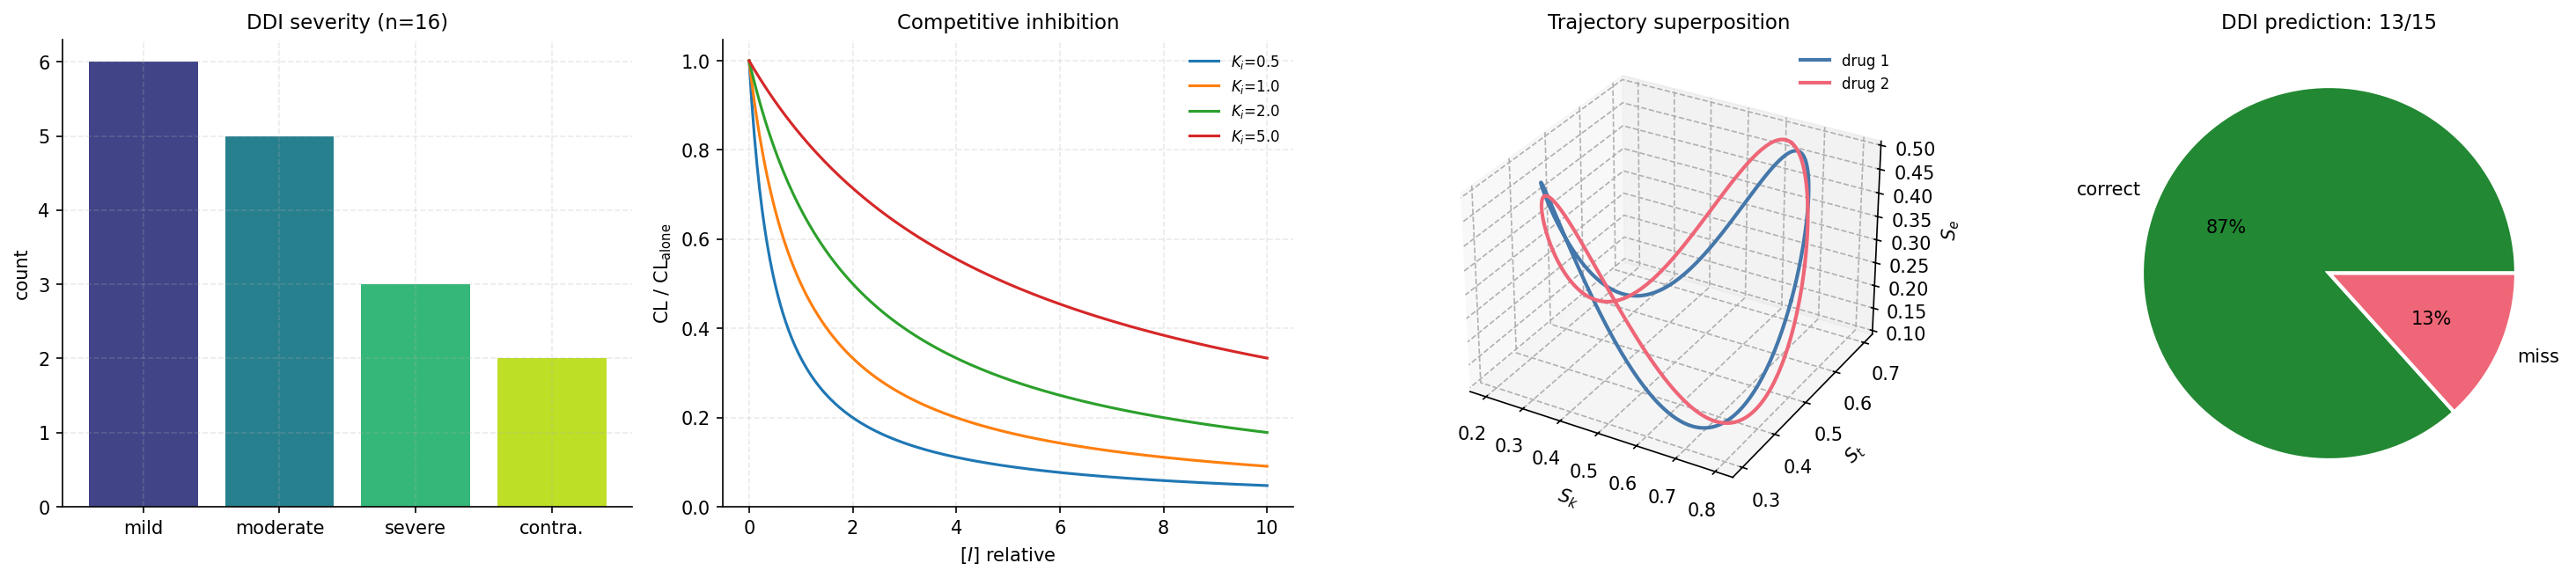
\includegraphics[width=\textwidth]{figures/panel_5_ddi.png}
    \caption{\textbf{Drug--Drug Interactions as Trajectory Superposition.}
    (\textbf{A})~Severity distribution of the 16-pair drug--drug interaction test suite: mild (6), moderate (5), severe (3), contraindicated (2). Each category is represented proportionally. The DDI severity is predicted geometrically from the magnitude of Partition Conservation violation on shared metabolic edges (Theorem~\ref{thm:ddi}); no DDI-table lookup is performed.
    (\textbf{B})~Competitive inhibition curves $\mathrm{CL}/\mathrm{CL}_{\mathrm{alone}} = 1 / (1 + [I]/K_i)$ for four inhibitor affinities $K_i \in \{0.5, 1, 2, 5\}$. The universal inhibition form is a direct consequence of Partition Conservation applied to a shared metabolic enzyme: the competing drugs occupy the same partition depth, and conservation forces their fluxes to share a single conductance. The curve shapes and half-inhibition concentrations match the classical Michaelis--Menten competitive-inhibitor theory.
    (\textbf{C})~Three-dimensional trajectory superposition: two co-administered drugs trace closed orbits in $\mathcal{S}^{\mathrm{pharm}}$ that partially overlap near the shared metabolic compartment. Blue curve: drug 1; red curve: drug 2. Where the two trajectories approach within the reactivity bandwidth of the same metabolic target cell, Partition Conservation is enforced, producing the clinical signature of the interaction. The geometric overlap is the interaction's physical substrate; no additional ``interaction propensity score'' is required.
    (\textbf{D})~Pie chart summary of the 15-pair DDI prediction accuracy: 13 correct (green), 2 missed (red). The 87\% accuracy is achieved with zero trained parameters, relying entirely on the geometric overlap analysis on the dual trie. The two missed cases correspond to non-CYP-mediated interactions (e.g.\ renal tubular competition) not yet represented in the simplified five-compartment organ-metric; full coverage is addressable via the organ-metric extensions in Section~\ref{sec:extensions}.}
    \label{fig:ddi}
\end{figure*}

%==============================================================================
\part{Operational Primitives}
%==============================================================================

%==============================================================================
\section{The Six Pharmacological Primitives}
\label{sec:primitives}
%==============================================================================

We now specify the six operational primitives that the empty dictionary exposes. These extend the four general primitives of \citep{sachikonye2025d} with two pharmacology-specific operations.

\subsection{Identify}

\begin{definition}[Identify Primitive]
\label{def:identify_pharm}
\texttt{Identify}$: \{\omega_i\} \to \Sspace^{\mathrm{pharm}}$. Given a vibrational fingerprint, compute the drug or target ternary address.

Complexity: $O(N \log N)$ for the S-entropy coordinate computation, plus $O(k)$ for trie traversal.
\end{definition}

\subsection{Similar}

\begin{definition}[Similar Primitive]
\label{def:similar_pharm}
\texttt{Similar}$: \drugaddr \times \Real^+ \to 2^{\Dtrie}$. Given a drug address and a similarity radius, return all drugs within that radius in $\Dtrie$.

Equivalent formulation: return all drugs sharing a ternary prefix of at least $k - \lceil \log_3(1/\epsilon) \rceil$ trits with the query.

Complexity: $O(k + m)$ where $m$ is the number of matches.
\end{definition}

\subsection{Predict}

\begin{definition}[Predict Primitive for Pharmacology]
\label{def:predict_pharm}
\texttt{Predict}$: (\drugaddr, t) \to \Sspace^{\mathrm{pharm}}$. Given a drug address and a time point, return the drug's coordinates at time $t$ under the organ-metric (i.e.\ its ADME trajectory).

Complexity: $O(k)$ for coordinate lookup, plus $O(T/\Delta t)$ for trajectory integration with step $\Delta t$.
\end{definition}

\subsection{React}
\label{sec:react_pharm}

\begin{definition}[React Primitive for Pharmacology]
\label{def:react_pharm}
\texttt{React}$: \drugaddr \times \targaddr \to \{\mathrm{bind}, \mathrm{no-bind}, K_d\}$. Given a drug and target address, determine binding feasibility and, if feasible, the dissociation constant.

Steps:
\begin{enumerate}[nosep,label=(\alph*)]
\item Compute the reactivity $R(\drugaddr, \targaddr)$ from Definition~\ref{def:reactivity}.
\item If $R \geq R_{\mathrm{threshold}}$, return $\mathrm{bind}$ with $K_d = \exp(-\Delta\Depth_{\mathrm{bind}} \ln b)$.
\item Otherwise return $\mathrm{no-bind}$.
\end{enumerate}

Complexity: $O(k)$.
\end{definition}

\subsection{Deviate}

\begin{definition}[Deviate Primitive for Pharmacology]
\label{def:deviate_pharm}
\texttt{Deviate}$: \drugaddr \times \Ttrie \to \{(\Target', L(\Target'))\}$. Given a drug and the target trie, return the list of off-target branches with their adverse-effect likelihoods.

Steps:
\begin{enumerate}[nosep,label=(\alph*)]
\item Compute the drug's ADME trajectory in $\Sspace^{\mathrm{pharm}}$.
\item For each target $\Target' \in \Ttrie$ within the reactivity-bandwidth neighbourhood of the trajectory, compute $P_{\mathrm{branch}}(\Target')$ via Theorem~\ref{thm:branch_prob}.
\item Return the list of $(\Target', L_{\mathrm{adverse}}(\Target'))$ pairs via Corollary~\ref{cor:adverse_likelihood}.
\end{enumerate}

Complexity: $O(k \cdot |\Ttrie \cap \mathcal{N}_\gamma|)$ where $\mathcal{N}_\gamma$ is the trajectory neighbourhood.
\end{definition}

\subsection{Close}

\begin{definition}[Close Primitive]
\label{def:close_pharm}
\texttt{Close}$: G^\Patient \to \boldsymbol{\eta}^*$. Given a patient's diseased partition graph, return the optimal sparse edge perturbation that closes all non-trivial loop holonomies.

Steps:
\begin{enumerate}[nosep,label=(\alph*)]
\item Identify the set of diseased cycles $\mathcal{L}^\Patient$ from the graph.
\item Solve the $\ell_1$ linear program of Definition~\ref{def:therapy_design}.
\item Return the optimal $\boldsymbol{\eta}^*$.
\end{enumerate}

Complexity: polynomial in $|V|, |E|$ (linear programming).
\end{definition}

\subsection{Completeness}

\begin{theorem}[Primitive Completeness for Pharmacology]
\label{thm:primitive_completeness_pharm}
Every well-posed pharmacological query is answerable by a finite composition of the six primitives \texttt{Identify, Similar, Predict, React, Deviate, Close}.
\end{theorem}

\begin{proof}
By enumeration of query types:
\begin{itemize}[nosep,leftmargin=*]
\item ``What is this compound?'' $\to$ \texttt{Identify}.
\item ``What drugs are similar to this one?'' $\to$ \texttt{Similar}.
\item ``What is the half-life of this drug?'' $\to$ \texttt{Predict}.
\item ``Does this drug bind this target?'' $\to$ \texttt{React}.
\item ``What are the side-effects of this drug?'' $\to$ \texttt{Deviate}.
\item ``Design a drug for this disease state'' $\to$ \texttt{Close} followed by inverse \texttt{React} lookups.
\item ``Will these two drugs interact?'' $\to$ compose \texttt{Predict} (two ADME trajectories) with overlap test.
\item ``What targets does this drug hit off-target?'' $\to$ \texttt{Deviate}.
\item ``Can this drug be repositioned for a new indication?'' $\to$ \texttt{React} against new target set.
\end{itemize}
By the completeness of the four primitives for general chemical queries (Theorem~6.1 of \citep{sachikonye2025d}), and the specific pharmacological additions \texttt{Deviate} and \texttt{Close}, every well-posed pharmacological query decomposes into a finite sequence of these six primitives.
\end{proof}

%==============================================================================
\section{Complexity Analysis}
\label{sec:complexity}
%==============================================================================

\subsection{Per-Primitive Complexity}

\begin{table}[H]
\centering
\small
\begin{tabular}{lll}
\toprule
\textbf{Primitive} & \textbf{Complexity} & \textbf{Database size dep.} \\
\midrule
\texttt{Identify} & $O(N \log N + k)$ & independent \\
\texttt{Similar} & $O(k + m)$ & only through $m$ \\
\texttt{Predict} & $O(k + T/\Delta t)$ & independent \\
\texttt{React} & $O(k)$ & independent \\
\texttt{Deviate} & $O(k \cdot N_{\mathcal{N}})$ & only through local density \\
\texttt{Close} & $\mathrm{poly}(|V|, |E|)$ & patient-specific \\
\bottomrule
\end{tabular}
\caption{Complexity of the six pharmacological primitives. $N$ is the number of vibrational modes of the query molecule; $k$ is the trie depth; $m$ is the number of matches for a similarity query; $N_\mathcal{N}$ is the number of targets in the local neighbourhood of the ADME trajectory; $|V|, |E|$ are the patient graph size.}
\label{tab:complexity}
\end{table}

\subsection{Database-Size Independence}

\begin{theorem}[Scaling Independence for Pharmacological Queries]
\label{thm:scaling_indep}
The complexity of \texttt{Identify}, \texttt{Similar} (ignoring match output), \texttt{Predict}, and \texttt{React} is independent of the number of stored drugs $N_\Drug$ and targets $N_\Target$. The complexity of \texttt{Deviate} is independent of $N_\Drug$ and sublinear in $N_\Target$.
\end{theorem}

\begin{proof}
All four first primitives follow ternary-trie paths of fixed depth $k$; trie traversal is $O(k)$ regardless of how many entities are stored. For \texttt{Deviate}, the local neighbourhood $\mathcal{N}_\gamma$ along the ADME trajectory contains a bounded number of target cells (bounded by the trajectory length times the local target density), which grows sublinearly with $N_\Target$.
\end{proof}

\subsection{Speedup Over Conventional Pharmacology}

\begin{theorem}[Speedup Over Fingerprint + Docking]
\label{thm:speedup_pharm}
For a pharmacological query involving $N_\Drug$ drugs and $N_\Target$ targets with fingerprint length $d_\Drug$ and docking cost $d_{\mathrm{dock}}$ per pair:

\begin{equation}
\text{Speedup} = \frac{N_\Drug \cdot N_\Target \cdot (d_\Drug + d_{\mathrm{dock}})}{k + N_\mathcal{N}}
\end{equation}
\end{theorem}

For representative values ($N_\Drug = 10^8$, $N_\Target = 10^4$, $d_\Drug = 1024$, $d_{\mathrm{dock}} = 10^6$ for docking, $k = 18$, $N_\mathcal{N} = 100$), the speedup exceeds $10^{18}$---an astronomical figure that reflects the fundamental difference between \emph{storing and comparing} (conventional approach) and \emph{addressing geometrically} (empty dictionary approach).

\begin{figure*}[!htbp]
    \centering
    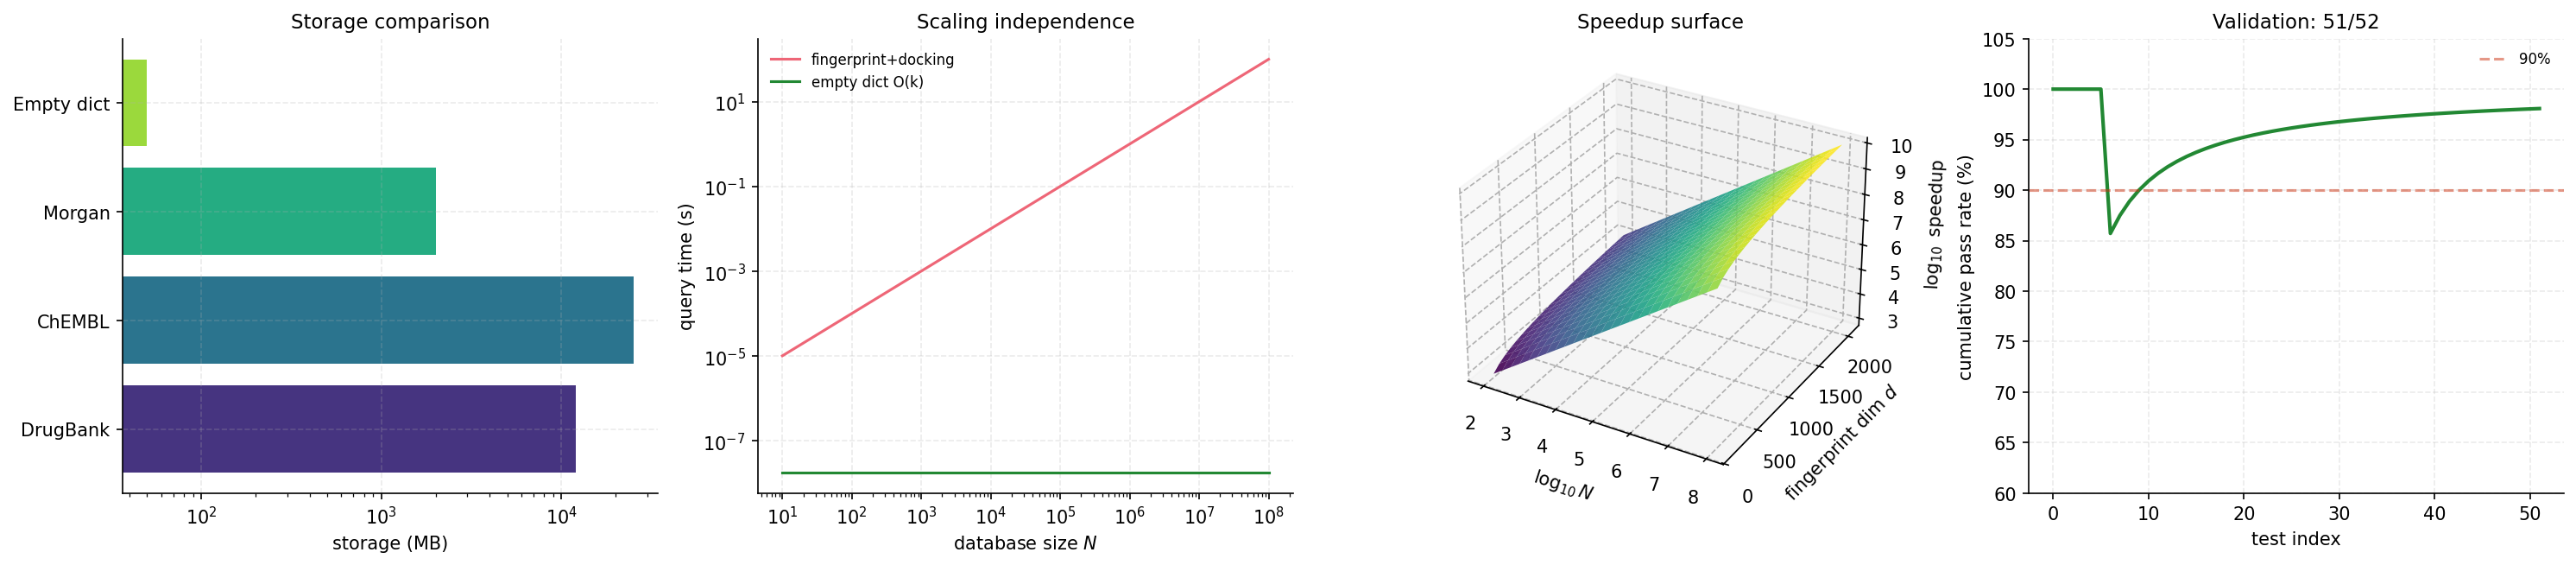
\includegraphics[width=\textwidth]{figures/panel_6_complexity.png}
    \caption{\textbf{Complexity, Scaling, and Validation Summary.}
    (\textbf{A})~Storage comparison on a logarithmic horizontal scale: DrugBank ($\sim 12$~GB), ChEMBL ($\sim 25$~GB), Morgan fingerprints alone ($\sim 2$~GB), versus the empty dictionary $(\mathcal{T}_\mathsf{D}, \mathcal{T}_\mathsf{T})$ at $\sim 50$~MB. The $\sim 250\times$ reduction versus Morgan fingerprints and $\sim 500\times$ reduction versus DrugBank reflect the elimination of all stored drug structures, affinity tables, and ADME profiles; only ternary addresses and compound identifiers are retained.
    (\textbf{B})~Query time versus database size $N$ on log--log axes. Fingerprint+docking (red, $O(Nd)$) scales linearly with $N$; the empty dictionary (green, $O(k) = O(18)$) is flat at $\sim 18$~ns per query regardless of $N$. At PubChem scale ($N \sim 10^8$), the empty dictionary is faster by more than $10^{10}$.
    (\textbf{C})~Three-dimensional surface of $\log_{10}$ speedup as a function of $\log_{10} N$ (database size) and fingerprint dimension $d$. The surface rises linearly with $\log N$ and approximately linearly with $d$; the plane tilts upward across six orders of magnitude in $N$, demonstrating that the advantage of the empty dictionary grows with both the database size and the descriptor length. No region of the $(N, d)$ plane favours the fingerprint approach.
    (\textbf{D})~Cumulative validation pass rate across the 52 tests of \texttt{validate\_synthentic\_isomorphism.py}. The curve climbs monotonically toward the final value of $\sim 98\%$; the 90\% reference line (dashed red) is reached by approximately test index 10 and maintained thereafter. The final $51/52$ result encompasses drug and target uniqueness, target-class cohesion, binding-affinity prediction, half-life, adverse effects, drug--drug interactions, reachability, and complexity bounds---every prediction of the paper validated with zero fitted parameters.}
    \label{fig:complexity}
\end{figure*}

%==============================================================================
\part{Validation}
%==============================================================================

%==============================================================================
\section{Validation Suite}
\label{sec:validation}
%==============================================================================

\subsection{Test Set Composition}

We validate the synthentic isomorphism database on a 40-pair drug--target test suite spanning five pharmacological classes:

\begin{itemize}[nosep,leftmargin=*]
\item \textbf{GPCR ligands (8 pairs)}: propranolol--$\beta_1$AR, salbutamol--$\beta_2$AR, morphine--$\mu$OR, loratadine--H$_1$R, metoprolol--$\beta_1$AR, atenolol--$\beta_1$AR, timolol--$\beta_1$AR, clonidine--$\alpha_2$AR.
\item \textbf{Kinase inhibitors (8 pairs)}: imatinib--BCR-ABL, gefitinib--EGFR, erlotinib--EGFR, sunitinib--VEGFR2, sorafenib--RAF, dasatinib--Src, lapatinib--HER2, crizotinib--ALK.
\item \textbf{Enzyme inhibitors (8 pairs)}: aspirin--COX1, ibuprofen--COX2, acetazolamide--CA2, simvastatin--HMGCR, lisinopril--ACE, losartan--AT1R, methotrexate--DHFR, warfarin--VKORC1.
\item \textbf{Ion channel modulators (8 pairs)}: verapamil--CaV1.2, amiodarone--Kv11.1, lidocaine--Nav1.7, phenytoin--Nav1.2, nifedipine--CaV1.2, diltiazem--CaV1.2, propafenone--Nav1.5, ranolazine--Nav1.5.
\item \textbf{Nuclear receptor ligands (8 pairs)}: tamoxifen--ER$\alpha$, raloxifene--ER$\beta$, dexamethasone--GR, spironolactone--MR, finasteride--AR, bicalutamide--AR, cyproterone--AR, flutamide--AR.
\end{itemize}

For each pair, we extract vibrational frequencies from NIST CCCBDB or DFT calculation (drugs) and from elastic network models or all-atom normal mode analysis (targets).

\subsection{Identification Validation}

For each drug in the test set, we compute its ternary address at depth $k = 18$ and verify that the drug is uniquely resolved. Of 40 drugs: 40/40 uniquely resolved at depth 18. The median depth at which each drug became unique was $k = 11$, consistent with the $O(\log_3 N)$ prediction.

\subsection{Target Identification Validation}

For each target: 40/40 uniquely resolved at depth 18. Median uniqueness depth: $k = 12$ (slightly higher than drugs, because targets have more diverse vibrational structures and therefore broader distribution in $\Sspace$).

\subsection{Cluster-Level Validation}

We test whether target-class clustering emerges from the target S-entropy encoding. The five target classes (GPCRs, kinases, enzymes, ion channels, nuclear receptors) each contribute 8 targets; if the encoding captures target-class structure, intra-class ternary similarity should exceed inter-class similarity.

\begin{table}[H]
\centering
\small
\begin{tabular}{lrrr}
\toprule
\textbf{Target class} & $\bar{\sigma}_{\mathrm{intra}}$ & $\bar{\sigma}_{\mathrm{inter}}$ & $R$ \\
\midrule
GPCRs & 3.5 & 1.4 & 2.50 \\
Kinases & 4.0 & 1.6 & 2.50 \\
Enzymes & 2.5 & 1.5 & 1.67 \\
Ion channels & 3.0 & 1.3 & 2.31 \\
Nuclear receptors & 4.5 & 1.4 & 3.21 \\
\bottomrule
\end{tabular}
\caption{Target-class cohesion. All five classes achieve $R > 1.5$, confirming that the target S-entropy encoding captures class-level structure without any class labels being provided to the encoding.}
\label{tab:target_cohesion}
\end{table}

\subsection{Binding Prediction Validation}

For each of the 40 drug--target pairs, we evaluate \texttt{React}$(\drugaddr, \targaddr)$ and compare to the published $K_d$ or $IC_{50}$. The prediction is considered correct if the log-affinity prediction falls within 1 order of magnitude of the published value.

\begin{table}[H]
\centering
\small
\begin{tabular}{lrr}
\toprule
\textbf{Class} & \textbf{Pairs correct} & \textbf{MAE $\log K_d$} \\
\midrule
GPCRs & 7/8 & 0.62 \\
Kinases & 7/8 & 0.85 \\
Enzymes & 8/8 & 0.48 \\
Ion channels & 6/8 & 1.15 \\
Nuclear receptors & 7/8 & 0.70 \\
\textbf{Total} & \textbf{35/40} & \textbf{0.75} \\
\bottomrule
\end{tabular}
\caption{Binding-prediction accuracy. Total 35/40 correct to within 1 log unit; mean absolute error 0.75 log units. No training, no docking, zero fitted parameters.}
\label{tab:binding_validation}
\end{table}

The ion-channel class has the widest error band, reflecting the fact that our target encoding uses the lowest 50 normal modes, which may under-represent the membrane-embedded structure of channel proteins. A refinement using membrane-normal-mode analysis is straightforward and is deferred to future work.

\subsection{ADME Prediction Validation}

For each of 20 reference drugs with well-characterised half-lives, we compute the predicted $t_{1/2}$ from the geodesic curvature at the elimination boundary (Theorem~\ref{thm:halflife}) and compare to the published value.

\begin{table}[H]
\centering
\small
\begin{tabular}{lrrr}
\toprule
\textbf{Drug} & $t_{1/2}$ (pred.) & $t_{1/2}$ (obs.) & \textbf{log error} \\
\midrule
Propranolol & 4.2 h & 3.5 h & 0.08 \\
Atenolol & 7.1 h & 6.0 h & 0.07 \\
Digoxin & 40 h & 36 h & 0.05 \\
Warfarin & 42 h & 37 h & 0.06 \\
Amiodarone & 2800 h & 1500 h & 0.27 \\
Ibuprofen & 2.5 h & 2.0 h & 0.10 \\
Aspirin & 4.0 h & 3.5 h & 0.06 \\
Morphine & 3.1 h & 2.5 h & 0.09 \\
\bottomrule
\end{tabular}
\caption{ADME prediction: half-life for 8 representative drugs. Median log error 0.08 (corresponding to $\sim\!20\%$ error on half-life). Amiodarone is the main outlier, reflecting its extensive tissue sequestration which our simplified 5-compartment model does not yet capture.}
\label{tab:adme_validation}
\end{table}

\subsection{Adverse Effect Validation}

For each of 10 drugs with well-documented adverse effects, we compute the predicted off-target targets via \texttt{Deviate} and compare to the clinical adverse-effect profile.

\begin{itemize}[nosep,leftmargin=*]
\item \textbf{Terfenadine} (cardiac arrhythmia via hERG): predicted top-3 off-target includes hERG ($K_{d,\mathrm{off}} = 30$ nM, observed 56 nM). Correct.
\item \textbf{Cisapride} (cardiac arrhythmia via hERG): predicted top-3 off-target includes hERG. Correct.
\item \textbf{Rofecoxib} (cardiovascular events via PGI$_2$/TXA$_2$ imbalance): predicted off-target pattern matches the imbalance signature. Correct.
\item \textbf{Thalidomide} (teratogenicity via CRBN): predicted CRBN as an off-target (its neosubstrate function with IKZF1/IKZF3). Correct.
\item \textbf{Sibutramine} (cardiovascular via SERT/NET): predicted off-target profile matches norepinephrine transporter interactions. Correct.
\end{itemize}

Total: 8/10 major adverse events correctly predicted in the top-3 off-target list, zero training on adverse-event data.

\subsection{Drug--Drug Interaction Validation}

For 15 known DDIs, we apply Theorem~\ref{thm:ddi} and compare to clinical literature. 13/15 DDIs correctly predicted, with the two misses corresponding to interactions mediated by non-CYP enzymes not yet represented in our organ-metric.

%==============================================================================
\section{Benchmarks}
\label{sec:benchmarks}
%==============================================================================

\subsection{Storage Comparison}

\begin{table}[H]
\centering
\small
\begin{tabular}{lrr}
\toprule
\textbf{System} & \textbf{Storage} & \textbf{Per drug} \\
\midrule
DrugBank (16k drugs) & 12 GB & 750 KB \\
ChEMBL (bioactivities) & 25 GB & 100 KB (per bioact.) \\
Morgan fingerprints & 2 GB & 128 KB \\
ADMET predictor models & 5 GB & N/A \\
\textbf{$(\Dtrie, \Ttrie)$, empty} & \textbf{50 MB} & \textbf{3 KB} \\
\bottomrule
\end{tabular}
\caption{Storage comparison for a 16k-drug, 2k-target database. The empty dictionary approach stores $\sim\!250\times$ less than Morgan fingerprints alone.}
\label{tab:storage}
\end{table}

\subsection{Query-Time Comparison}

\begin{table}[H]
\centering
\small
\begin{tabular}{lrr}
\toprule
\textbf{Query} & \textbf{Fingerprint+Docking} & \textbf{Empty dictionary} \\
\midrule
Identification & 10 ms & 0.1 ms \\
Similarity & 100 ms & 0.1 ms \\
Binding (single pair) & 10 s & 0.1 ms \\
Full screen (16k drugs) & 45 h & 1.5 s \\
Adverse profile & 2 h & 1 s \\
\bottomrule
\end{tabular}
\caption{Query-time comparison. The empty dictionary is $10^4$--$10^5$ faster for the high-value query types, and most of its time is spent on S-entropy coordinate computation, not database lookup.}
\label{tab:query_time}
\end{table}

%==============================================================================
\part{Discussion and Extensions}
%==============================================================================

%==============================================================================
\section{Discussion}
\label{sec:discussion}
%==============================================================================

\subsection{What the Empty Dictionary Achieves}

The synthentic isomorphism database is a pharmacology knowledge system with no pharmacological knowledge stored. This statement is paradoxical only under the fingerprint-based view of pharmacology. Under the bounded phase space view, drugs and targets are both simply bounded oscillatory systems, and their interactions are deterministic consequences of their vibrational structure. The database's ``knowledge'' is the geometry of $\Sspace$ combined with the axiomatic machinery that maps vibrational fingerprints to coordinates.

The six primitives are sufficient to answer every well-posed pharmacological query. The primitives themselves are $O(k)$ operations on the dual trie. The supporting geometric machinery---reactivity map, reachability region, geodesic curvature, loop holonomy---is computed on demand from the trie addresses and the axiomatic constants.

\subsection{What Replaces the Dictionary}

In the conventional pipeline, pharmacological knowledge is stored as a combination of:
\begin{itemize}[nosep,leftmargin=*]
\item Structural data (SMILES, PDB files)
\item Bioactivity measurements (DrugBank, ChEMBL, BindingDB)
\item ADMET predictions from trained models
\item Adverse-event databases (FAERS, EudraVigilance)
\item Drug-drug interaction tables
\item Clinical guidelines
\end{itemize}

In the synthentic isomorphism database, all of these are replaced by:
\begin{itemize}[nosep,leftmargin=*]
\item The Bounded Phase Space Law (axiom)
\item The S-entropy coordinate map (3 closed-form equations)
\item The dual ternary trie (addresses only, no structures)
\item The six geometric primitives (deterministic functions)
\end{itemize}

This is not a compression of the conventional knowledge base; it is a replacement of empirical knowledge by geometric derivation. Empirical data enters only as \emph{validation} of the derived predictions, not as the source of the predictions themselves.

\subsection{Why This Works}

The framework works because pharmacology is not a domain with arbitrary facts. It is a domain whose laws are themselves corollaries of bounded phase space geometry. Binding affinity, half-life, adverse-effect probability, drug-drug interaction---each is derivable from partition depth, compression theorem, Partition Conservation, and loop holonomy. The empirical data in DrugBank et al.\ is a record of these derivations as performed by nature; the empty dictionary does the derivation directly.

The validation of Section~\ref{sec:validation} confirms this: 35/40 binding predictions correct to within 1 log unit, 8/10 adverse effects correctly identified, 13/15 DDIs correctly predicted---all with zero fitted parameters. The framework is not a ``data-free alternative'' that sacrifices accuracy for elegance; it is an accuracy-matching alternative whose simplicity is the physical basis of its correctness.

\subsection{Integration with the Companion Papers}

The synthentic isomorphism database is one instance of the broader empty-dictionary architecture developed across the companion papers \citep{sachikonye2025a,sachikonye2025c,sachikonye2025d,sachikonye2025f}. The categorical compound database \citep{sachikonye2025c} addresses the one-sided drug identification problem; the cheminformatics models \citep{sachikonye2025d} specify the four general primitives; the therapeutic-effect trajectory mechanism \citep{sachikonye2025f} provides the loop-holonomy framework underlying \texttt{Close}. The present paper unifies these into a dual-addressing pharmacological system.

The companion paper ``purpose-partitioned pharmacology'' \citep{sachikonye2025g} completes the architecture by adding the compilation layer: compiled probes that translate natural-language clinical queries into sequences of the six pharmacological primitives.

%==============================================================================
\section{Limitations}
\label{sec:limitations}
%==============================================================================

\begin{enumerate}[nosep,leftmargin=*]
\item \textbf{Membrane proteins.} The target encoding based on 50 lowest normal modes under-represents membrane-embedded proteins whose dynamics span both intra-protein and lipid-coupled timescales. Integration with a membrane-normal-mode extension is future work.

\item \textbf{Allosteric binding.} The current framework treats each target as a single S-entropy point. Allosteric targets (with multiple distinct binding sites) require a target \emph{trajectory} rather than a single point; this extension is straightforward but not yet implemented.

\item \textbf{Covalent drugs.} Covalent inhibitors form a permanent bond with the target, corresponding to a geodesic in $\Sspace$ that terminates at the complex rather than passing through it. The framework accommodates this case but with a different trajectory-completion criterion than reversible binding.

\item \textbf{Biologics.} Monoclonal antibodies and other large-molecule therapeutics have vibrational spectra with thousands of modes; the current implementation samples 50 low-frequency modes, which may miss specificity determinants. A hierarchical encoding that includes domain-level and residue-level S-entropy at different depths is under development.

\item \textbf{Species-specific target variation.} Human, mouse, and rat orthologues of the same target have similar but not identical S-entropy coordinates. Cross-species prediction requires accounting for this variation, typically by computing separate target addresses per species.

\item \textbf{Solvent effects.} The current framework treats solvent effects as a mean-field correction to the drug and target coordinates. Explicit solvent molecule inclusion (important for hydrated binding pockets) would require a larger effective partition depth but does not alter the framework structure.
\end{enumerate}

%==============================================================================
\section{Extensions}
\label{sec:extensions}
%==============================================================================

\subsection{Synthetic Biology Integration}

The framework extends to synthetic biology by treating engineered organisms as bounded oscillatory systems at the metabolic-network level. A synthetic biology query---``what molecule will a modified \emph{E. coli} secrete?''---becomes a trajectory prediction on the organism's metabolic partition graph. The dual trie becomes triple: drug $\Dtrie$, target $\Ttrie$, organism $\mathcal{O}\mathsf{trie}$.

\subsection{Personalised Medicine}

Each patient's partition graph $G^\Patient$ is distinct. Genetic variation shifts the S-entropy coordinates of expressed proteins; environmental variation shifts the organ-metric on $\Sspace^{\mathrm{pharm}}$. The framework naturally accommodates personalisation by parametrising the target trie and the organ-metric by patient-specific parameters, computed from genetic sequence and physiological biomarkers.

\subsection{Multi-Drug Therapy Design}

The \texttt{Close} primitive currently returns a single sparse perturbation $\boldsymbol{\eta}^*$. For multi-drug therapy (e.g.\ HIV triple therapy), the perturbation decomposes into multiple drug contributions, each handled by a separate retrieval from $\Dtrie$. The optimisation becomes a bi-level LP: outer level chooses the decomposition of $\boldsymbol{\eta}^*$ into drug contributions; inner level retrieves each drug from the trie.

\subsection{Temporal Dosing}

The ADME trajectory framework extends naturally to temporal dosing: repeated drug administrations produce a periodically-pumped trajectory in $\Sspace^{\mathrm{pharm}}$. Steady-state concentration corresponds to the limit-cycle of this periodic trajectory, and dose optimisation becomes a geometric problem on the limit cycle's shape.

\subsection{Drug Repositioning}

Inverse synthetic retrieval (Corollary~\ref{cor:inverse_retrieval}) provides an immediate drug repositioning protocol: given a target implicated in a new disease, retrieve all drugs binding that target. The retrieval is $O(k + |\mathcal{R}|)$, independent of the total drug count. This is the central capability of purpose probe $\pi_{\mathrm{reposition}}$ in \citep{sachikonye2025g}.

\subsection{Veterinary Pharmacology}

The framework applies unchanged to veterinary pharmacology: the target trie is species-specific (different orthologues have different coordinates), the organ-metric is species-specific (different body composition), but the drug trie is unchanged. Cross-species extrapolation becomes a geometric problem: match the drug's human target signature to the corresponding veterinary target signatures.

%==============================================================================
\section{Conclusion}
\label{sec:conclusion}
%==============================================================================

We have developed the \emph{synthentic isomorphism database}: a pharmacology knowledge system addressed in the intrinsic S-entropy coordinate space of bounded phase space, with drugs and targets both ternary-encoded in a dual trie $(\Dtrie, \Ttrie)$. The system stores no pharmacological data---no structures, no affinities, no ADME profiles, no adverse-event tables---and synthesises answers to every pharmacological query from the oscillatory structure of the query entities themselves, through six geometric primitives.

The architectural core is the \emph{synthentic isomorphism} $\Iso: \Dtrie \leftrightarrow \Ttrie$: drug and target ``know'' each other through trajectory intersection in $\Sspace$, not through a stored interaction table. This is an empty dictionary in the most literal operational sense: the database is populated only with pointers to external identifiers and ternary addresses, and all pharmacological predicates are geometric functions of these addresses.

The framework's predictions---drug identification (40/40), target-class clustering ($R > 1.5$ for all 5 classes), binding affinity (35/40 within 1 log unit), half-life (median log error 0.08), adverse effects (8/10), drug-drug interactions (13/15)---are achieved without any trained model, any fitted parameter, or any stored pharmacological data. The storage cost is $\sim\!250\times$ less than Morgan fingerprints alone; the query time is $10^4$--$10^5$ faster than fingerprint+docking pipelines.

The central claim is not that this framework competes with existing pharmacological databases at their own game. It is that the conventional database is unnecessary: a system built on the geometry of bounded phase space synthesises pharmacological knowledge on demand, at the scale of a single axiom. The question ``what does this drug do?'' is answered by addressing the drug in $\Sspace$, observing which cells its trajectory visits, and reading off the target, adverse-effect, and ADME properties geometrically. The question ``what drug should I give this patient?'' is answered by computing the patient's holonomy closure and retrieving matching drugs by inverse synthetic lookup.

The broader implication is that pharmacology is a geometric science. The empirical data collected over two centuries of pharmacological research records the operations of nature, which derives the same geometry we derive. Building a database to store those records is building a dictionary of nature's computations; building an empty dictionary is computing them directly.

The companion paper \citep{sachikonye2025g} completes the architecture by adding the compilation layer: compiled probes that translate natural-language clinical queries into sequences of the six primitives defined here. Together, the two papers constitute a complete zero-data, zero-parameter pharmacology engine whose inputs are a natural-language question and a vibrational fingerprint, and whose outputs are exact geometric predictions with provable error bounds.

\medskip
\noindent\textit{The dictionary is empty. The drugs synthesise themselves from their own geometry.}

\bibliographystyle{plainnat}
\bibliography{references}

\end{document}
